\documentclass[11pt]{report}
\usepackage{baththesis}
\usepackage{graphicx}
\usepackage[T2A]{fontenc}
\usepackage[utf8]{inputenc}
\usepackage{caption}
\usepackage{amsmath}
\usepackage{latexsym}
\usepackage{multirow}
\usepackage{multicol}
\usepackage{subcaption}
\usepackage{verbatim}
\usepackage[inline]{enumitem}
\usepackage{paralist}
%\usepackage{amsfonts}
\usepackage{url}
\usepackage{natbib}
\usepackage[hmargin=3cm,vmargin=2cm]{geometry}
%\usepackage{mathpazo}
%\usepackage{eulervm}
\usepackage[usenames,dvipsnames,svgnames,table]{xcolor}
\usepackage[]{todonotes}
\usepackage{tikz}
\usetikzlibrary{arrows}
\usepackage[]{todonotes}

\newcounter{myenumi}
\setcounter{myenumi}{0}
\newenvironment{myenumerate}{\begin{compactenum} \setcounter{enumi}{\themyenumi}}{ \setcounter{myenumi}{\theenumi}\end{compactenum}}

\def\mnote#1{\todo[color=Goldenrod,size=\scriptsize]{Matt: #1}}
\def\jnote#1{\todo[color=CornflowerBlue,size=\scriptsize]{Julian: #1}}
\def\snote#1{\todo[color=WildStrawberry,size=\scriptsize]{Steve: #1}}
\definecolor{light-gray}{gray}{0.95}
\def\tropical{TropICAL}

\usepackage{listings}
\lstset{ %
   language=prolog,
%  frame=l,                     % adds a frame around the code
   basicstyle=\footnotesize\ttfamily,  % use courier
   breaklines=true,
   xleftmargin=0.5em,
   aboveskip=0.5em,
   belowskip=0.5em,
%  belowcaptionskip=5em,
   numbers=left,
   backgroundcolor=\color{light-gray},
   frame=single,
   framerule=0pt
}

\setlength{\jot}{0pt}
\def\mylabel#1{\tikz[remember picture]\node(#1){};}
\def\myref#1#2#3{\begin{tikzpicture}[remember picture]
\node[draw,rounded corners] (#2){\begin{minipage}{\textwidth}\raggedright#3\end{minipage}};
\draw[overlay,-triangle 45,thick,gray](#2.west)--(#1.west);
\end{tikzpicture}}

\title{Building Abstractable Story Components with Institutions and Tropes}
\author{Matt Thompson}
\degree{EngD Digital Media}
\department{Department of Computer Science}
\degreemonthyear{October 2016}
\norestrictions


\begin{document}

% ----------------------------------
% \maketitle

% \clearpage
% \tableofcontents
% \clearpage

% \begin{abstract}
% This report summarises the research carried out as part of the EngD Digital Media programme with the University of Bath and Sysemia Ltd.

% The purpose of this report is to explain the academic research conducted during the course and its applicability to the needs of Sysemia Ltd. The main focus is to explore the state of the art in interactive and generative narrative and also to apply it in a real-world exhibition context.
% \end{abstract}

% ----------------------------------

% intro
% \chapter{Introduction}
\label{cha:introduction}
The central contribution of this thesis is the use of story tropes for the
generation of structured, interactive narratives for use in games, training
simulations or other playable experiences. In order to introduce the research
described in later sections, this introduction will first explain the concepts of story
tropes and interactive narrative.

\section{Story Tropes}

Story tropes are recurring motifs in the narratives of media, which allow for a more expressive manner of describing stories than existing narrative formalisms. Authors can use them to build new story components and re-use existing tropes to make hierarchical story arcs.

Tropes describe commonly-seen themes and elements of stories. In a sense, they are similar to clich\'es, in that an audience becomes familiar with them through repeated exposure. However, tropes are not clich\'es. Clich\'es are story elements that have been repeated ad nauseum, that are so often used and unoriginal that they evoke tedium from their audience. Tropes may perhaps become clich\'es if they are used to the point of becoming tiresome, though some are so embedded into the collective subconscious that their presence is taken for granted. Joseph Campbell argues that \emph{The Hero's Journey} is a trope that transcends time and culture, representing a shared human blueprint for the rite-of-passage into adulthood~\cite{campbell2008hero}. In this way, stories and tropes could be considered a cultural language for describing common human themes. Clich\'es could not be described as such: they are simply overexploited ideas.

The themes, scenes, characters and structure of a story can be described in terms of tropes. Even individual lines of dialogue can be a trope, such as James Bond's witty put-downs when he defeats an enemy. Tropes describe parts of a story in an abstract way, which means that they can be easily identified in multiple stories.

Examples of tropes are:

\begin{compactitem}
\item \textbf{The Hero's Journey}: A hero answers a call to adventure, and leaves home to go on a journey. They defeat the villain along the way, returning back home triumphant.
\item \textbf{The Evil Empire}: The villain is part of an empire, which tries to stop the hero at all costs.
\item \textbf{The MacGuffin}: There is an object that the hero needs, the search for which is used to drive the plot.
\item \textbf{Chekhov's Gun}: If a gun appears somewhere in the first act, it must be fired by the end of the third.
\end{compactitem}

Tropes can describe a story at several layers of abstraction, meaning that tropes can contain other tropes as sub-tropes. For example, \emph{The Hero's Journey} can contain the \emph{Hero}, \emph{Quest}, and \emph{Call to Adventure} sub-tropes. This allows a degree of expressivity unavailable in other narrative models described in the \emph{Related Work} section.

In interactive narrative generation, where a player may take one of many possible paths through a story, parts of the story are often procedurally generated in order to save an author the time and effort of manually writing out all the branches of the narrative. However, this means that the author must give up some control over the structure and content of the story. By describing the intended contents of the story in an abstract manner using tropes, an author is able to give it structure. In our case, the procedural generation occurs through the use of intelligent agents to model story characters. These character agents are guided towards pursuing actions that fit the tropes in the authored narrative, thus gently making sure they meet the expectations of the author while allowing them some degree of freedom with which to pursue their own goals.

\section{Interactive Narrative}
Interactive narratives have the potential to transform two major fields: games
and training simulations. These are the applications for which the use of
interactive narrative can benefit Sysemia. The main part of the research examines the state of the art in interactive narrative primarily in computer games research, but then adapts techniques from that field for the purpose of interactive exhibitions. By implementing research ideas into `toy' game projects (such as an interactive Punch and Judy show in section \ref{sec:pj}), I then take components from these projects and implement them into practical exhibition-based projects for Sysemia (such as the Every Object Tells a Story project described in section \ref{sec:every}).

Though media such as computer games allow a player to influence events through interaction with its characters and objects, the story of the game itself is usually predetermined. In order to create media in which the narrative is shaped by a person's interactions, one two approaches are usually taken: emergent narratives or branching narratives.

\textbf{Emergent narratives} occur when a story (of sorts) unfolds as a result of a player's interactions with the rules of the game world. Examples of this appear in the games \emph{Minecraft}, \emph{Civilisation}, \emph{Dwarf Fortress} and \emph{The Sims}. In these cases, no author has sat down and written a branching narrative for every eventuality in the game. Instead, the narrative is created by the story world itself in response to a player's actions.

The advantage of this type of narrative is easily apparent from an author's point of view: it saves them the work of having to write all the branches of a story. In a story with any nontrivial amount of branching, the author would have to spend a great many hours writing down all of the alternative paths through it. In the end, a player might not even see the result of a fraction of the effort put into a game's writing. An emergent story solves this problem by procedurally generating a narrative.

However, it could be argued that these emergent stories are only ``stories'' in the loosest possible sense --- they have no shape or structure, no recurring motifs, and nothing like a climax near the end. They do not take the player on an emotional ride, but merely describe a sequence of events. Indeed, it greatly decreases the influence of the writer as an artist, leaving a story totally in the hands of the player. If a game author has a certain story they want to tell in a non-linear fashion, or a message that they wish to convey, they must resign themselves to hoping that it somehow emerges from the unscripted interactions of a player with the game.

\textbf{Branching Narratives}, on the other hand, give authors total control over what happens in a non-linear story. They are able to structure each possible branch of the narrative, ensuring some branches terminate in climaxes while others lead to despair. They can insert artistic themes into their stories, and put their own personal flourishes into every single aspect of it. The price of this control is the amount of work it requires for the creation of each story branch, as well as the limited amount of branching an author's time constrains them to write.

Ideally, we could combine the best features of both type of non-linear narrative: the labour-saving generative element of emergent narratives and the structural control of the branching narratives.

\section{Interactive narrative for games}
Computer games are a new medium for artistic expression. The element of interactivity, combined with visual art, music and storytelling, allows the creation of ever more fantastic worlds. This combination of previous art forms isn't enough, though. Game creators are now experimenting with ways to make a narrative itself interactive. Imagine playing through a version of Romeo and Juliet where there is a possibility that the characters could escape their fates. Or playing a detective in a game where the story changes depending on how quickly you can piece together clues.

This is the new frontier that we are exploring with this research: the as-yet unconquered domain of \emph{interactive} storytelling.

We are defined by the choices we make throughout our lives. These choices form a story that describes our own personal history. If a player can watch somebody's life unfold and witness the choices that they made, and those that were forced upon them, they would have a deep understanding of how they came to be who they are.

This kind of deep understanding is only possible through experiencing a story where the decisions made have real consequences. Traditional fiction, and perhaps computer games, enable this to some extent. But the story is still experienced passively by the consumer in these media. A truly interactive narrative would go deeper, as though you had truly lived as another person.

For this reason, interactive narrative for games is worth exploring: it would
enable a player to truly understand other people's lives and situations, and why they became the people they are.

% Put a bit about what you did to explore the potential of interactive narrative
% for games

\section{Interactive narrative for education}
Stories are a powerful way for humans to understand and remember facts and events. Making these stories interactive could lead the way to even more effective learning methods.

\citet{schank1990tell} argues that stories may be a useful way for humans to better remember a series of events, when compared to simply reciting them as a list of facts. Mentalists and creative students use storytelling mnemonic techniques to help them memorise large lists of difficult-to-remember facts with perfect recall.

Training simulations make the use of stories taking place in immersive environments to help trainees to master new routines and techniques. These stories always follow a fixed pattern, however, unlike the mnemonic stories that people create to memorise information, which are highly personalised to the practitioner.

A narrative that dynamically reacts to the decisions of the audience could better enable them to remember information when compared with a static, unpersonalised narrative.

With this in mind, it is worth constructing an interactive narrative system and applying it to both entertainment and learning contexts. Some evaluation still needs to be carried out in order to determine how much more effective (if at all) interactive narrative could be for education, so this is proposed as part of this report.

Preliminary work has been done in collaboration with the Bishop's Palace in Wells to create an exhibition incorporating interactive narrative. Using a combination of Semantic Web data formats and an event calculus-based reasoner, the system will be able to infer future actions for recommendation to visitors. Description of the work done so far is in section \ref{sec:nthsn}.

Both the game-based and education-based projects have a common thread: reasoning
over temporal data in order to predict future events, or constrain possible
future actions to conform to a narrative domain. Section \ref{sec:nthsnt}
describes the direction the research has taken, and how the use of techniques such as hierarchical institutions and the creation of an ontology for narrative might develop these ideas further.


\section{Outline}
% Outline of sections goes here
This thesis begins with a review of the literature in Section~\ref{cha:literature-review}. This review covers two main fields of research: narrative research from social science (Section~\ref{sec:narratology}), and interactive narrative research from computer science (Section~\ref{sec:implementations}).
The ``Institutions as Story Worlds'' chapter (\ref{cha:institutions}) describes the theory and research behind instituitions, and discusses the merit of their use for describing story, comparing their use against other logics and planner-based systems.
The ``Tropes as Story Components'' chapter (\ref{cha:tropes}), discusses the use
of \emph{tropes} as story components, and why they improve upon existing narrative formalisms.
Chapter~\ref{cha:tropes-and-institutions} describes how to use institutions to define tropes, and how to combine them to describe the story world for an interactive narrative. The section also describes the use of this technique to build a number of different narratives, contrasting the approach with using other techniques such as planners to build interactive narratives.
The final chapter looks back at the research done, evaluating its potential impact and discussing possible future work. 


% litrev
% \chapter{Literature Review}
\label{cha:literature-review}

This research covers multiple fields of study such as narratology, interactive
storytelling, emotional modelling and artificial intelligence, therefore an extensive
literature review covering these fields is necessary. This section starts with a
look at the field of \emph{narratology}, or narrative theory, to gain some
insights into the themes and components that make up stories. Looking at
different formalisms that have been created for narrative and which themes and
motifs recur in stories should better inform the creation of techniques with
which to generate stories.

We also examine current approaches to interactive narrative generation,
focussing particularly on the use of planners, drama managers, social norms and
logical modelling for describing stories. Most of these implementations are
designed with multi-agent systems in mind, where the story forms a set of rules
which govern these agents. The start of this part of the literature survey also
examines non-interactive story generation through means of techniques such as
generative grammar, in order to provide a historical context for the research
that follows. 

As part of the examination of implementations of interactive narrative, this review especially focuses on agent-based systems. The section concludes with an overview of emotional models that can be used to model distinct characters using agents.

\section{Narratology}
\label{sec:narratology}
Narratology is a deep field with many sub-fields. This review examines the parts of it that might best inform the modelling of narrative by computers, as well as the construction of interactive narrative.

The first part of the overview of narratology examines research into categorising different types of narrative, both traditional and experimental.
This draws from classic narratological texts, as well as work done on
``cybertext'' and experimental narrative in the interactive age. This
examination of recent research into non-linear narratives is essential for the
construction of interactive narratives for games or simulations.

Structuralist formalisms of narrative attempt to explain how stories work by dividing them into commonly occuring themes and motifs. This is a natural fit to the modelling of narratives by computer. This overview of narratology starts with structuralism for this reason.

After the overview of structuralists' narrative models there follows a section on the use of formal logic for narrative modelling. The section ends with descriptions of other types of story components, taxonomies and ontologies used in the literature.

\subsection{Narrative Structure}
\label{sec:structure}
What is the difference between a narrative and a sequence of events? If we
recount the events that happened to us during the course of a day, would that
``count'' as a narrative? When is the retelling of events a simple listing of
facts, and when is it a story?

Narratologists from \citet{bal2009narratology} onwards refer to the
chronological ordering of events as \emph{fabula} (from the Russian фабула, ``scene''), and the retelling and
reordering of those events in a narrative as \emph{syuzhet} (сюжет, ``plot'').
In fact, Russian structuralists~\citet{propp1968morphology} and~\citet{shklovsky1991theory} were the first to use these terms in the
context of narrative, before their rediscovery by modern narrative theorists.

The concepts of \emph{fabula} and \emph{syuzhet} are key to the understanding of
narrative structure. Thanks to Aristotle's
\emph{Poetics}~\citep{halliwell1986aristotle}, we understand that a story must
have a beginning, a middle and and end. These three parts of a story describe
how the \emph{syuzhet} are organised, which can refer to its \emph{fabula}
(chronological) events in any order. For example, the beginning of a movie could
be set at the present day in the life of the protagonist, the middle could be a
flashback to an earlier time in her life, and the end could return to the events
following the start of the movie.

Though Aristotle identifies the beginning, middle and end as three key story
divisions, other theorists divide the \emph{syuzhet} of a story further. Joseph
Campbell's work \emph{The Hero with a Thousand Faces}~\citep{campbell2008hero}
describes how almost every story is a variation of the \emph{Hero's Journey}
(which Cambell also calls the \emph{monomyth}). Like Aristotle's beginning, middle and end,
the Hero's Journey has three acts: the Departure, the Initiation and the Return.
Campbell divides these acts further into seventeen distinct stages:

\paragraph{Departure}
\begin{myenumerate}
  \item The Call to Adventure
  \item Refusal of the Call
  \item Supernatural Aid
  \item Crossing the Threshold
  \item Belly of the Whale
\end{myenumerate}
\paragraph{Initiation}
\begin{myenumerate}
  \item The Road of Trials
  \item The Meeting with the Goddess
  \item Woman as Temptress
  \item Atonement with the Father
  \item Apotheosis
  \item The Ultimate Boon
\end{myenumerate}
\paragraph{Return}
\begin{myenumerate}
  \item Refusal of the Return
  \item The Magic Flight
  \item Rescue from Without
  \item The Crossing of the Return Threshold
  \item Master of Two Worlds
  \item Freedom to Live
\end{myenumerate}

In summary, the hero begins the story at home or in some otherwise familiar
setting, where she is called away on an adventure. After possibly rejecting this
call, the hero leaves home (crosses the threshold) and sets off for the land of adventure. After facing
many trials and possibly defeating an enemy, the hero returns home once again.
Having endured the many trials of the journey, our hero becomes stronger in spirit
and character.

As a classic example, consider the plot of Tolkien's \emph{The Hobbit}. At the
start of the tale, Bilbo Baggins is a comfortable but risk-averse hobbit who
refuses to leave his comfortable surroundings when Gandalf first visits to
send him on a quest. Of course, he does eventually leave home to fulfill the
quest, returning home a changed character.

Campbell argues that the \emph{monomyth} acts as a shared cultural memory of
sorts, being the universal template for the rite-of-passage tale. He says that
it is passed down as myth through many different cultures, replicating in much the same way
as genes (or memes) do and that it can be thought of as a \emph{metamyth}, or the
spiritual history of humanity.

% Polti 27
% Look at story shapes paper for inspiration
Other analysts have described several different types of commonly-seen plot.
\citet{harris1959basic} makes the case for just three types of plot, having
either a happy ending (where the protagonist is virtuous), an uphappy ending
(with a selfish protagonist) or being a tragedy (where the protagonist is struck
by fate).

\citet{booker2004seven} describes seven basic plots, where each may have either a
happy or unhappy ending:
\begin{compactitem}
  \item Overcoming the monster
  \item Rags to riches
  \item The quest
  \item Voyage and return
  \item Comedy
  \item Tragedy
  \item Rebirth
\end{compactitem}

Georges Polti famously divides narratives into the \emph{thirty-six dramatic
  situations}~\citep{polti1921thirty}, derived from his analysis of classical
Greek and both classical and contemporary French texts. Polti's thirty-six types
of plot are:

\begin{multicols}{2}
\begin{compactenum}
  \item Supplication
  \item Deliverance
  \item Crime pursued by vengeance
  \item Vengeance taken for kin upon kin
  \item Pursuit
  \item Disaster
  \item Falling prey to cruelty/misfortune
  \item Revolt
  \item Daring enterprise
  \item Abduction
  \item The enigma
  \item Obtaining
  \item Enmity of kin
  \item Rivalry of kin
  \item Murderous adultery
  \item Madness
  \item Fatal imprudence
  \item Involuntary crimes of love
  \item Slaying of kin unrecognized
  \item Self-sacrifice for an ideal
  \item Self-sacrifice for kin
  \item All sacrificed for passion
  \item Necessity of sacrificing loved ones
  \item Rivalry of superior vs. inferior
  \item Adultery
  \item Crimes of love
  \item Discovery of the dishonour of a loved one
  \item Obstacles to love
  \item An enemy loved
  \item Ambition
  \item Conflict with a god
  \item Mistaken jealousy
  \item Erroneous judgment
  \item Remorse
  \item Recovery of a lost one
  \item Loss of loved ones
\end{compactenum}
\end{multicols}

\begin{figure}[!t]
\centerline{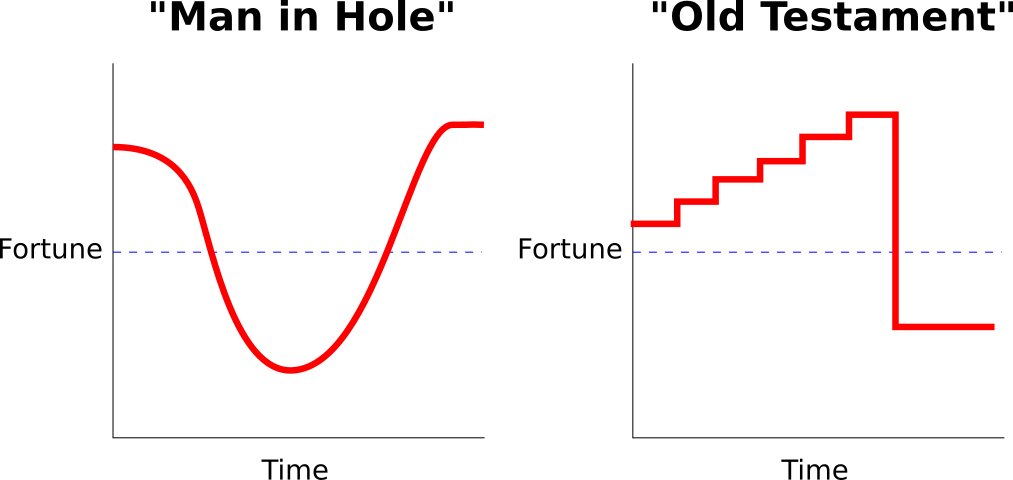
\includegraphics[height=2in]{vonnegut.png}}
\caption{Two of Kurt Vonnegut's ``Shapes of Stories''}\label{fig:vonnegut}
\end{figure}

Author Kurt Vonnegut describes several different ``shapes'' of stories in his
rejected Master's thesis~\cite{vonnegut2009palm}. He plots the events of a story
as points in a 2D space with ``Beginning-End'' (time) on the X-axis and ``Ill
Fortune-Great Fortune'' (fortune of protagonist) on the Y-axis.
Figure~\ref{fig:vonnegut} shows two examples of story shapes. In the ``Man in
Hole'' example, things start out well for the story's protagonist, but then some
misfortune falls on them. They spend much of the story overcoming challenges
before finally ending the story with a triumph. In the ``Old Testament''
example, the protagonist(s) experience gradually increasing levels of fortune,
before finally being ``cast down'' to a grave level of misfortune at the end of
the story.

All of the above categorisations describe stories as a whole, sorting narratives
into one of several different ``types'' of story. This works well for
linear narratives within traditional media, but what about experimental and
non-linear narratives? In the next section, we review the literature relating to
these less traditional types of stories.

\subsection{Types of Narrative}
% Author Kurt Vonnegut
% Look at Cybertext, etc, and try to explain how best to divide different types
% of story
The rise of the Web in the 1990s brought with it great interest in the future of narrative in cyberspace. Aarseth's work, \emph{Cybertext} \citep{aarseth1997cybertext} describes the creation of a new form of narrative, for which he coins the term \emph{ergodic literature} (from the Greek words \emph{ergon} and \emph{hodos}, meaning `work' and `path'). In this new form of narrative, some amount of work or effort is required by the reader in order to traverse the path that the story takes.

% scriptons/discourse textons/fabula (Bal 1997)
Aarseth makes a distinction between the narrative as written by the author, and the way in which it is traversed by the reader, calling the former \emph{textons} and the latter \emph{scriptons}. In ergodic literature, the \emph{scripton} is produced by the effort that the reader goes through in interpreting the \emph{texton}. In the context of a game, it is as though the game interface is a gateway that allows access to the narrative at different times. Using classical music as a metaphor, the texton can be thought of as the \emph{score}, and the scripton the \emph{performance}.

% TODO Make sure you update the intro with this
In section~\ref{sec:generative-and-interactive-narrative}, we assert that how generative a narrative is and its level of interactivity are two different variables in an experimental narrative. However, Aarseth identifies seven different methods of story traversal: \emph{dynamics, determinability, transiency, perspective, access, linking and user function}.

\textbf{Dynamics} describe whether or not the content and number of scriptons changes. In a simple, static story with branching choices (such as in a \emph{Choose your own adventure} story), both the number of textons and scriptons are fixed, since all paths have been written out beforehand. A dynamic story would still have a fixed number of textons, but the scriptons would be generated as the user traverses the path of the narrative.

\textbf{Determinability} is how deterministic the narrative is, whether or not the same interactions will result in the same scripton being produced.

\textbf{Transiency} means to what extent scriptons are produced as time flows, or whether user interactions are required to produce them.

\textbf{Perspective} is whether or not the user/reader plays a role as a character in the narrative.

\textbf{Access:} if a user has access to all scriptons at any point in traversing the narrative, or whether their access is restricted.

\textbf{Linking:} whether or not parts of the scripton are linked to other parts, and whether these links are conditional (if they rely on a user having already traversed part of the scripton).
\textbf{User functions:} the functions the user uses to traverse the text. This could be interpretive (which is implicit in any traversal of the text), explorative (traversing the scripton according to whim) or configurative (specifying parts of the scripton in advance), for example.

% Ugh, this is all so arbitrary. Go on to describe Aarseth's PCA of these variables and explain why you don't think it's a good fit.

By performing correspondence analysis (a process similar to principle component analysis) on a diverse corpus of 23 texts ``\emph{ranging from ancient China to the Internet}'', Aarseth filters these seven variables down into two numerical axes which account for 49 percent of the variation between stories. Using these axes, he groups classic tales such as \emph{Moby Dick} and more experimental narratives such as William Gibson's \emph{Agrippa} and Michael Joyce's \emph{Afternoon}. By grouping these stories into categories, he intends to show how emerging media are enabling new types of story.

Chris Crawford's \emph{Chris Crawford on Interactive Storytelling} \citep{crawford2012chris} provides a scathing assessment of the relationship between narrative theory and computer science. A veteran of the games industry, he argues that `soft' science theories such as those of Aarseth et al are entirely removed from `hard' science, and are therefore an example of bubble intellectualism and impossible to implement. 

Crawford himself provides a useful examination of experimental narrative in computer games, defining interactivity as:

\begin{quote}
A cyclic process between two or more active agents in which each agent alternately listens, thinks, and speaks.
\end{quote}

He argues that for game narratives to be truly interactive, they must be more social. Characters in a story must be able to react with the player as though they were people in real life. In turn, the player should have some degree of freedom in the way in which they interact. Rather than presenting branching story points as choices, a better way to interact would be socially, through talking to agents in the game. This is the approach that Fa\c{c}ade takes \citep{mateas2003faccade}, which Crawford acknowledges as the most successful attempt at interactive storytelling to date. A detailed description of Fa\c{c}ade's implementation appears in section \ref{sec:modelling-agents}.

In order to determine whether Crawford's assertion that narratology research is
too far removed from its practical implementations to be of use, we provide an
overview of these implementations and their underlying research in section \ref{sec:implementations}. Has narrative theory research informed the creation of computer-generated or interactive narrative at all, or do they all take approaches grounded in computer science and artificial intelligence? If narrative theory has not been used, then we must ask: why not?


\subsection{Structuralist Formalisms of Narrative}
% Propp, etc
Attempts to organise recurring themes, roles and motifs of narrative go back at least a century. The Aarne-Thompson tale-type index \citep{aarne1987types}, first published in 1910 and later refined by Stith Thompson in 1928 and 1961, is well known amongst folklorists as a classification and analysis method for traditional folktales and myths. Aarne-Thompson's index is a taxonomy of tale themes, arranging tales into categories such as \emph{animal tales} and \emph{jokes and anecdotes}, and then sub-categories (\emph{tales of magic} and \emph{numskull [sic] stories} being two examples). This taxonomy is only two levels deep however, and only serves as a useful way to categorise individual stories or tales. In order to break down and analyse components of tales, we must dig deeper.

In \emph{Structural Anthropology}, Claude L\'{e}vi-Strauss seeks to discover why myths and legends are so similar across cultures and history \citep{levi1963structural}. He concludes that there are global laws that govern the way in which people create stories, therefore these laws can be modelled as a set of rules for describing myths.

His theory is that myths describe opposing forces which are resolved through mediation. The example he gives in \emph{Structural Anthropology} describes how Native American legends often contain `trickster' characters in the form of ravens or coyotes. As scavenging animals, these tricksters symbolically act as mediators between life and death.

Like much of early narrative theory, there is no rigorous evaluation of L\'{e}vi-Strauss' ideas, leaving them seeming opinionated and arbitrary. While interesting, L\'{e}vi-Strauss' ideas bring us no closer to developing a formal model of narrative structure. For that, we must go even further back in time, and turn to Vladimir Propp.

\subsubsection{Propp's Morphology of the Folktale}
A notable narrative structuralist is Vladimir Propp, creator of \emph{The Morphology of the Folktale}~\citep{propp1968morphology}, a formalism for Russian folktales. Propp's formalism, though originally limited in scope, generalises well, and is still used by researchers to procedurally generate stories~\citep{grasbon2001morphological,gervas2005story,hartmann2005motif}. Drawing from a corpus of one hundred Russian folktales, Propp identifies thirty-one distinct \emph{story functions}, each of which is identified by a number and symbol. These functions are executed by characters following certain roles, each of which has a \emph{sphere of action} consisting of the functions that they are able to perform at any given point of the story. Stories are created by chaining story functions together, with subplots expressed as parallel chains of story functions.

In this formalism, characters have \emph{roles}, such as \emph{hero}, \emph{villain}, \emph{dispatcher}, \emph{false hero}, and more. Characters performing a certain role are able to perform a subset of \emph{story functions}, which are actions that make the narrative progress. For example, the \emph{dispatcher} might send the \emph{hero} on a quest, or the \emph{victim} may issue an \emph{interdiction} to the \emph{villain}, which is then \emph{violated}.

Propp defines a total of 31 distinct story functions, each of which is given a number and symbol in order to create a succinct way of describing entire stories. Examples of such functions are:

\begin{compactitem}
  \item One of the members of a family absents himself from home: \emph{absentation}.
  \item An interdiction is addressed to the hero: \emph{interdiction}.
  \item The victim submits to deception and thereby unwittingly helps his enemy: \emph{complicity}.
  \item The villain causes harm or injury to a member of the family: \emph{villainy}.
\end{compactitem}

Each of these functions can vary to some degree. For example, the \emph{villainy} function can be realised as one of 19 distinct forms of villainous deed, including \emph{the villain abducts a person}, \emph{the villain seizes the daylight}, and \emph{the villain makes a threat of cannibalism}.

\begin{figure}[!t]
\centerline{
\includegraphics[height=0.4in]{propp1.png}}
\caption{One Propp function following another}\label{fig:propp1}
\end{figure}

\begin{figure}[!t]
\centerline{
\includegraphics[height=0.6in]{propp2.png}}
\caption{Multiple simultaneous functions}\label{fig:propp2}
\end{figure}

In a typical story, one story function will follow another as the tale progresses in a sequential series of cause and effect (figure~\ref{fig:propp1}). However, Propp's formalism also allows for simultaneous story functions to be occuring at once (figure~\ref{fig:propp2}).

Though flexible, Propp's formalism is limited in its expressiveness. All story functions describe events at the same level of abstraction, describing one event after another. Also, Propp insists that the story functions occur in a prescribed order. Later French structuralists such as \citet{bremond1980logic}, \citet{greimas1983structural} and~\citet{todorov1969grammaire} address the latter problem by generalising Propp's work outside of Russian Folktales, though each represents only incremental improvements on Propp, lacking a means of nesting story functions to create abstractions. \citet{barthes1975introduction} broadly describe hierarchically composing \emph{narrative units} but, lacking implementation details, these can only be used as a template from which to build a new narrative model.
% What are the shortcomings of Propp? (i.e. lack of abstractability, etc)

% \subsection{Describing Stories with Logic}
% Laure-Ryan did a bit of this, also include linear logic approaches

\subsection{Other Types of ``Story Component''}
Lehnert's \emph{plot units} are a more recent narrative formalism
\cite{lehnert1981plot}. However, these plot units only describe stories as three
types of event: positive, negative and mental. These events occur with respect
to a single character in the story, so an author must always author story
components with concrete characters in mind, making them difficult to re-use.
Similar to Propp's system, the order of composition must always be in a certain
sequence, and plot units cannot refer to other plot units. Again, we are left
without a means of creating abstractions for our story components. In the
``TropICAL: a DSL for Tropes'' section, we address this issue by describing how tropes allow the nesting of components to allow story authors to create their own abstractions.

\section{Implementations of Experimental Narrative}
\label{sec:implementations}
% I've plenty of material, but it really needs reworking and extending

\subsection{Story Generation}
% TaleSpin, etc
Inspired by Chomsky's theories of generative grammar \citep{chomsky1968sound}, researchers in generative narrative strive to build their own `universal grammar' for narrative.

\begin{figure}[!t]
  \begin{center}
  \begin{compactenum}
    \item $\texttt{Attempt}\rightarrow \texttt{Plan} + \texttt{Application}$\\
           $\qquad\Rightarrow\texttt{MOTIVATE(Plan, Application)}$
    \item $\texttt{Application}\rightarrow\texttt{(Preaction)*} + \texttt{Action} + \texttt{Consequence}$\\
           $\qquad\Rightarrow\texttt{Allow(AND(Preaction,Preaction,...),}$\\
           $\qquad\{\texttt{CAUSE | INITIATE | ALLOW}\}\texttt{(Action,Consequence)}$
  \end{compactenum}
  \end{center}

  \caption{Example rules from Rumelhart's story grammar}\label{fig:rumelhart}
\end{figure}

\citet{rumelhart1975notes} provides one early and influential model for the grammatical generation of natural language. Figure \ref{fig:rumelhart} shows two example rewrite rules from this grammar. The `+' symbol denotes items happening in a sequence, the `\textbar' showing possible alternatives. `*' denotes one or more item being generated. Capitalised words (such as ALLOW, MOTIVATE, etc) describe relationships between items. For example, MOTIVATE is a relationship between a character's thought and their reaction to that thought.

Other systems draw inspiration from generative grammar, such as GESTER \citep{pemberton1989modular}, which generates stories based on a grammar synthesised from old French epic tales. \citet{lang1999declarative} describes a declarative model for narrative, consisting of lists of first-order predicate calculus expressions. These expressions describe events, states, goals and beliefs which combine to form a narrative. More specifically, it combines:

\begin{compactitem}
  \item A \textbf{grammar interpreter} to search for a sequence of grammar rewrites which would produce a convincing narrative.
  \item A set of \textbf{temporal predicates} to describe the occurence of events over time and enforce temporal constraints on story components.
  \item A \textbf{world model} which describes the set of actions that characters may perform and fluents that may alter over the course of the narrative.
  \item A \textbf{natural language output unit}, which takes the sequence of events produced by the story grammar and converts it into readable natural language sentences.
\end{compactitem}

This combination of using a grammar interpreter, world model and natural language output unit is especially common amongst generative grammar approaches.

While generative grammar approaches may be effective for procedurally creating
prose, they are less well suited to the creation of \emph{interactive}
narratives. Once the grammar rewrite rules are specified, the user is entirely
passive, unable to affect the way in which the story is being generated. For
this to happen, the narrative needs to be part of a system that reacts to the
actions of the user, such as in a computer game.

\begin{figure}[!t]
\begin{quote}
  ONCE UPON A TIME GEORGE ANT LIVED NEAR A PATCH OF GROUND. THERE WAS A NEST IN AN ASH TREE. WILMA BIRD LIVED IN THE NEST. THERE WAS SOME WATER IN A RIVER. WILMA KNEW THAT THE WATER WAS IN THE RIVER. GEORGE KNEW THAT THE WATER WAS IN THE RIVER. ONE DAY WILMA WAS VERY THIRSTY. WILMA WANTED TO GET NEAR SOME WATER. WILMA FLEW FROM HER NEST ACROSS THE MEADOW THROUGH A VALLEY TO THE RIVER. WILMA DRANK THE WATER. WILMA WASN'T THIRSTY ANYMORE.

GEORGE WAS VERY THIRSTY. GEORGE WANTED TO GET NEAR SOME WATER. GEORGE WALKED FROM HIS PATCH OF GROUND ACROSS THE MEADOW THROUGH THE VALLEY TO A RIVER. GEORGE FELL INTO THE WATER. GEORGE WANTED TO GET NEAR THE VALLEY. GEORGE COULDN'T GET NEAR THE VALLEY. GEORGE WANTED TO GET NEAR THE MEADOW. GEORGE COULDN'T GET NEAR THE MEADOW. WILMA WANTED TO GET NEAR GEORGE. WILMA GRABBED GEORGE WITH HER CLAW. WILMA TOOK GEORGE FROM THE RIVER THROUGH THE VALLEY TO THE MEADOW. GEORGE WAS DEVOTED TO WILMA. GEORGE OWED EVERYTHING TO WILMA. WILMA LET GO OF GEORGE. GEORGE FELL TO THE MEADOW. THE END.
\end{quote}
\caption{Example TALE-SPIN output}\label{fig:tspin}
\end{figure}

% TODO elaborate on this
James Meehan's TALE-SPIN \citep{meehan1977tale} is an influential early approach to story generation using planning. In TALE-SPIN, the author describes a story domain, its characters and their goals, and a natural language story is produced as output. It works by using a problem-solver to resolve each character's goals over the story domain. Figure \ref{fig:tspin} is an example of TALE-SPIN's output.

TALE-SPIN's strong planning component is evident in the reading of its output. Sentences are terse, with one event leading directly to another in order to achieve some goal. One problem with this character-led approach is that the goals of the author are not necessarily taken into account. If the author intends for a character to die at some point in the story, it seems unnatural for a character to have the goal of dying to fulfill this intention.

 Turner criticises TALE-SPIN's stories as seeming ``pointless and somewhat boring'' \citep{turner1986thematic}, going on to create the MINSTREL system for story generation \citep{turner1993minstrel}. Using the legendary world of King Arthur's court as a story domain, MINSTREL strives to generate stories with an authorial purpose.

MINSTREL attempts to address TALE-SPIN's shortcomings by introducing two types of schema: author-schemas and character-schemas, both of which combine to represent the elements of a story. The author-schemas describe the goals of the author of the system, allowing story creators more control over the structure and content of their narrative. This allows authors to specify a `point' or moral to their story, something that is not possible to achieve with TALE-SPIN. Character-schemas describe character-level goals in a similar manner to those of TALE-SPIN's.

The comparison of TALE-SPIN and MINSTREL highlights a challenge that has
dominated story generation for decades: the balance of \emph{character} and
\emph{plot} (as~\citet{riedl2010narrative} highlights). Especially with approaches based on multi-agent systems, the regulation of character actions to conform to an underlying theme or structure is a challenging problem.

However, modelling characters with agents is a promising approach to take in order to achieve a story which is both generative and interactive. In such a system, an author can specify the story world and character models, creating the `big picture', and the agents would be able to fill in the details (such as dialogue, sub-plots, and relationships).
An apt metaphor would be that of animation. In large animation studios such as
Disney, the lead animator draws the key frames of a sequence, and a team of
other animators work to fill in the gaps in
between\footnote{This process is described at the following website:
  \url{http://www.justdisney.com/animation/animation.html}, accessed 20160805.}. This is what the combination of a managed narrative with agents could achieve: the author would be the `lead animator' in such a system, with the agents being the assistants.

The implementations until now have focused mainly on \emph{generation\/}, and little on \emph{interaction\/}. Character models have been mentioned, but these do not react in real time to a user. For that, we need a multi-agent system.

\subsection{Characters as Intelligent Agents}
Story worlds are usually populated with characters. Interactive story worlds
such as games contain characters with very basic scripted behaviour. At even the
highest level of game character simulation, AI techniques are usually used to
govern basic behaviour such as movements and actions. Governing character
behaviour to fit within the context of a narrative is a more challenging
problem. This section examines different approaches to tackling this challenge.

\subsubsection{Planner-based Systems}
The most prevalent approach to the generation and management of plot in
interactive narrative is to use planners. With a planner, an author sets the
goals for the story (certain situations that they would like to see happen), and
the planner tells the character agents what to do to make sure these ``story
goals'' are achieved. When a player that is interacting with the system takes an
action that compromises the story goals, the planner must re-plan to make sure
the goals can still be achieved, by restricting the actions of the player or
intervening in some other manner.

% This needs elaboration
\citet{young1999notes} argues that planners are a good method for regulating
plot, later creating the \emph{Mimesis} architecture for integrating a planner with character agents in an interactive game environment, \citep{young2004architecture}. Young describes how narrative systems must re-plan when a player makes  narrative-breaking actions, by either restructuring the narrative mid-story (\emph{accommodating} the action) or preventing the action from executing (\emph{intervening} on the action).

Given its influence over subsequent approaches to interactive narrative
generation, it is worth looking at the Mimesis architecture more closely.
It is designed to integrate into the \emph{Unreal
  Tournament} game engine, and has five components: the \emph{mimesis
  controller}, the \emph{story planner}, the \emph{discourse planner}, the
\emph{execution manager} and the \emph{MWorld}.

Figure \ref{fig:mimesis} shows how these components work together to form the
Mimesis architecture. Once an author has created the pre-defined libraries of
actions needed by the story planner, the following steps are taken to determine
the course of the story:

\begin{compactenum}
  \item All the components connect to the Mimesis Controller (MC) via socket
    connection. It then acts as a message router.
  \item The game initiates a plan request containing the state of the game
    world, a list of possible actions, and the goals for the plan.
  \item The \emph{story planner} responds with a \emph{story world plan}, a data
    structure that describes the actions (selected from the list) that must occur over time in order to
    meet the plan request's goals.
  \item Once the story world plan is created, it is sent to the \emph{discourse
      planner}, along with a list of actions that can occur in the game engine
    (such as camera movements, voice-overs and background
    music). The discourse planner then creates a sequence of these actions that
    best fit the story world plan.
  \item The discourse planner then sends the narrative plan to the
    \emph{execution manager}, which builds a directed acyclic graph (DAG), where
    the nodes are the actions within the plan and the edges are the temporal
    constraints between the orderings of the actions. The execution manager
    removes nodes from the DAG in order, sends the node's actions to the
    game engine, and updates the graph.
  \item The \emph{MWorld} is essentially the environment in which the story
    occurs, consisting of the game engine, coordination code, and class
    definitions for actions, and discourse planners. It is the MWorld that
    receives actions from the execution manager to be executed, and executes
    these actions in the game engine.
\end{compactenum}

Mimesis uses DPOCL (Decomposed Partial-Order Causal-Link Planner,~\citep{young1994decomposition}) plans for
its story planning. DPOCL plans are composed of \emph{steps} (the plan's
actions), \emph{ordering constraints}, \emph{decomposition links} describing the
hierarchical structure of a plan, and \emph{causal links} between pairs of
steps. It uses \emph{refinement search} \citep{kambhampati1995planning} as its
plan reasoning process, searching through the space of possible plans represented as a directed
graph, with each node in the graph being a plan or partial plan. Mimesis
specifies the initial planning problem for DPOCL using the current and goal
states of the story.

A key feature of Mimesis is its strategies for handling of user actions which potentially
interfere with the story plan, making its goals unachievable. In the intervention strategy, Mimesis simply prevents the
user's action from having any effect in the game world. With accommodation,
Mimesis replans the story events, restructuring the plan so that the interfering
actions are taken into account and worked around.

\begin{figure}[!t]
\centerline{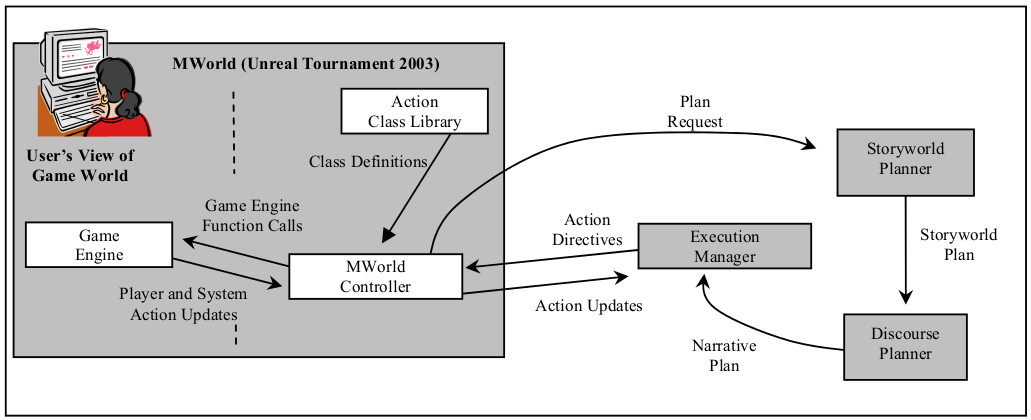
\includegraphics[height=2in]{mimesis.png}}
\caption{The Mimesis architecture, from \cite{young2004architecture}}\label{fig:mimesis}
\end{figure}

% This needs elaboration
\citet{cavazza2002character} et al's \emph{I-Storytelling} system implements
\citet{young2004architecture}'s architecture with ideas from Barthes' narrative
units~\citep{barthes1975introduction}, using characters with behaviour described
by Hierarchical Task Networks (HTNs) to generate its stories. Each character has a main task, which is divided into subtasks to create a task hierarchy, with each task node having pre- and post-conditions. The story emerges from the outcomes of each character's plans, and the narrative structure as a whole is not planned.

% This needs elaboration
\citet{riedl2003managing} describes a further development of Young's architecture,
allowing the story author to create plans for the overall narrative in addition
to its characters.
Rather than using a narrative model, this version of Mimesis models the player to track their expected level of suspense while interacting with the story. Like the \emph{I-storytelling} system, its plans are hierarchical, using the Longbow hierarchical partial-order causal link planning system~\citep{young1994decomposition}.

A disadvantage of these planner-based systems is that they require the story
author to think in a planner-oriented manner. They must consider the goals of
both the story and the character, plans to achieve these goals, and re-planning
when goals are not met or when situations change. This is a drastic change from
the usual story writing methods of authors, where the focus is on structure,
plot, themes and characters. Though graphical user interfaces such as Mimesis'
Bowman system~\citep{thomas2006author} could be used to assist plan-driven
story authoring, a complete shift in creative workflow is still required, making
this approach inaccessible to non-technical writers.

% This needs elaboration
\subsubsection{Drama manager-based Systems}

Carnegie Mellon University's OZ project \cite{mateas1999oz} uses a \emph{drama manager} to structure its narrative, which observes the actions occurring in the storyworld and ``directs'' its characters to conform to shape the story. 

Mateas and Stern's \emph{Fa\c{c}ade} has players interact with the characters of the story through natural language. In this game, the player attends the party of a young couple (Grace and Trip) celebrating their wedding anniversary. As the course of events unfold however, the player learns that all is not as happy as it seems.

The player interacts with the characters by typing in natural language sentences, to which Grace and Trip respond. Though the characters are implemented through agents, the story is controlled using a drama manager. In all, their system consists of using NLP, a novel character authoring language and a novel drama manager to create an interactive narrative.

Several custom-designed languages were used to create the game, including a language called `A Behaviour Language' (ABL) for the agents and a special language for the sequencing of the beats. ABL represents situations as character goals, maintaining a tree of all the active goals and behaviours that are happening at any time.

In Fa\c{c}ade, the smallest unit of narrative action is called a \emph{story beat}, taken from McKee's book on authorial style for screenwriters \citep{mckee1997substance}. The simulation constantly monitors what the user is doing and how it may lead from the current story beat to another. Story beats have preconditions and effects on the state of the narrative, so it is the drama manager's job to work out when it makes sense to initiate a certain beat.

`Beats' have a very fine granularity, with 200 or so updating every minute of the simulation. They consist of a set of ABL behaviours, which advance the narrative yet still allow interaction to change to other beats. Only one beat can be active at a time.

A beat can have 5 types of goal:

\begin{compactenum}
  \item transition-in: characters express their intentions
  \item body: a dramatic question/situation is posed to the player
  \item local/global mix-in: react to the player before end of the beat
  \item wait-with-timeout: wait for the player's reaction
  \item transition-out: final reaction to the player's action in the beat
\end{compactenum}

A beat goal is a series of steps for an agent to perform, which can be:

\begin{compactitem}
  \item staging (where to walk to, face)
  \item dialogue to speak
  \item where and how to gaze
  \item arm gestures to perform
  \item facial expression to perform
  \item head and face gestures to perform
  \item small arm and head emphasis motions triggered by dialogue (head nods, hand flourishes)
\end{compactitem}

As an example, there is a behaviour called ``Fix\_Drinks'', which specifies a sequence of agent behaviours where the characters Grace and Trip have an argument while Trip asks the player what they would like to drink. If the player decides not to go along with the beat (in this case, by not choosing a drink), then the beat will be aborted and replaced with another.

Fa\c{c}ade has become popular as a game outside of academia, with playthroughs of the game reaching millions of views on Youtube. This shows the promise of interactive narrative as being a unique and engaging new form of entertainment. Unfortunately, no other implementation of interactive narrative seems to have captured the public imagination since the release of Fa\c{c}ade.

Fa\c{c}ade's popularity seems to reinforce Crawford's assertion (section \ref{sec:media}) that interactive narratives must be social in nature. The gameplay comes entirely from the conversations and interactions between Grace, Trip and the player. Much of the excitement comes from the social consequences of certain conversation paths or actions. By modelling characters as agents, Mateas et al have created a truly interactive experience. However, by also using a drama manager to manage the agents, they have used these agents to tell a story.

How might these agents be made more convincing? Outside of writing rules for their behaviour consisting of character goals and beliefs, how might an author create truly unique and idiosyncratic characters? To address the question, I next examine different types of emotional models in psychology, and how each might be used to model characters as agents.

\subsubsection{Social Norms}
Versu~\cite{evans2014versu} is an interactive drama system that uses a multi agent system as characters. The characters' actions are coordinated with \emph{social practices}, which describe types of social situations and is described by the authors as a successor to the Schankian script. These social practices are implemented as reactive joint plans, which agents can choose to participate in or not. Rather than directly telling the agents what to do, these social practices merely \emph{suggest} courses of action, leaving each agent to decide for itself what to do based on its individual goals.

The authors decide against using a drama manager to control the agents' actions because they want to take the \emph{strong autonomy} approach to agent governance. This means that they prefer to give each agent some degree of autonomy by allowing it to make the final decision on which course of action to take, rather than blindly following a drama manager. Suggesting actions with social norms achieves this goal. Rather than describing typical story events in terms of social norms, however, in Versu the social norms \emph{are} the story. The gameplay revolves around the avoidance (or purposeful subvertion of) awkward social situations.

Each character has a role, which is governed by a social practice. For example, a \emph{greeting} practice involves characters with the \emph{greeter} and recipient roles. The greeting practice would tell the greeter in which manner they are to greet the recipient, and the recipient how to respond. It is noteworthy that these actions are merely suggested, and not enforced.

\emph{Exclusion logic}~\cite{evans2010introducing} is used to describe the
social practices of the system. Exclusion logic manages the frame problem by
organising related fluents in a tree structure. A single update at the right
branch can change a set of related facts en masse. For example, a description of a character called ``Brown'' is shown in listing \ref{lst:exclusive}. It describes the building up of character attributes as a tree structure.

Exclusion logic aims to address the frame problem. The frame problem is the uncertainty around whether predicates that change over time (fluents) change other predicate values. It aims to address this through use of an exclusion operator (``!''). Listing \ref{lst:exclusion} shows an example of the exclusion operator in use. The example specifies that an agent can have only one gender. The \emph{Praxis} language implementation of the exclusion logic has a type checker which ensures that no character can have multiple genders.

\begin{lstlisting}[float,label=lst:exclusion,caption=nextHopInfo: caption]
A(agent).sex!G(gender).
\end{lstlisting}

\begin{lstlisting}[label=lst:exclusion,caption=Description of ``Brown'' character.]
brown.sex!male;
brown.class!upper;
brown.in!dining_room;
brown.relationship.lucy.evaluation.attractive!40;
brown.relationship.lucy.evaluation.humour!20.
\end{lstlisting}

Exclusion logic's exclusion operator allows an author to express the fact that a variable can only have one value. For example, if `the `Brown'' character changes location from the dining room to the kitchen, \emph{brown.in!dining\_room} is terminated when \emph{brown.in!kitchen} holds.

Versu takes the \emph{constitutive} view of social practice, as opposed to the
\emph{regulative} view~\citep{SJP:SJP658}. This means that rather than restricting an agent's possible actions based on its permissions and obligations, they participate in a certain social practice by taking an action. Their actions are only restricted by what is possible in the story world, and what the agent desires to do. This way, agents can choose whether or not to take part in certain social interactions.

Many of the components we aim to have in our story telling system appear in Versu: the use of social norms to gently encourage story-conforming behaviour rather than demanding it, and the use of formal logic to determine which behaviours are possible. However in Versu the social norms \emph{are} the story, rather than describing the story components that invisibly govern the behaviour of characters. In order for this kind of governance to occur, an institution-based solution is preferable, based on events, agent actions and standard deontic logic. Because character actions are constrained by the structure of a story, a \emph{regulative}  view of social practice is more suited to the expression of story components as social norms.

Many of the advantages of using exclusion logic can be gained by using an institution-based approach. Non-inertial fluents can be used to ensure that variables can only ever have one value. Standard deontic logic is enough to provide the rest of what is needed.

% Need at least one more example here
\subsection{Modelling Narrative with Logic}
\label{sec:model-logic}
Although most recent research focuses on the use of planners to manage the drama in a story, there is also much interesting work which makes use of formal logic to model narrative. Though often used for the generation of linear story text, it is increasingly being applied to non-linear narratives as well. Logic-based approaches are generally based on either temporal logic variants or some kind of linear logic.

Ceptre~\citep{martens2015ceptre} is a language for modelling generative interactive narratives using \emph{linear logic}, a formal logic designed to describe resource usage. 

A Ceptre story begins with an initial state $\Delta_0$. Each state iteration
$\Delta_i$ is examined repeatedly, and a subset $S$ of it is updated with rule
$r$. The next state, $\Delta_{i+1}$, has the subset $S$ replaced with $S'$, the
new subset with the consequences of the applied rule $r$.

The rules are specified using the combination of logical statements with two
operators: $*$ (tensor) and $\text{-o}$ (lolli). The tensor operator is used to
concatenate statements, while the lolli operator expresses state transitions in
the form $S \mathrel{\text{-o}} S'$. The rules use \emph{replacement semantics},
which means that everything from state $S$ will disappear unless stated to be in
state $S'$. A $\$$ operator is used to mark facts in $S$ that the author wishes
to remain in $S$ without explicitly stating so.

Listing \ref{lst:ceptre-murder} shows an example from~\cite{martens2015ceptre}
that describes a ``murder'' rule and its consequences.

\begin{lstlisting}[label=lst:ceptre-murder]
do/murder
    : anger C C' * anger C C' * anger C C' * anger C C' *
    $at C L * at C' L * $has C weapon
    -o !dead C'.
\end{lstlisting}

In this case, four instances of the ``anger'' predicate with the same arguments
has a significant meaning: a character's emotion is treated as a resource. The
fact that \emph{anger $C C'$} appears four times means that a character is
\emph{four times} as angry at another character. Depending on how many times the
``anger'' statements appear in the new state, this anger can rise or fall at the
next step in the story. In this case, the emotion is not only treated as a
pre-condition, but also as a resource. These resources can also be specified
through the addition of a number to the name of the resource.

Ceptre introduces a \emph{stages} feature that allow authors to structure a
program through the use of independent components. A stage is a unit of
computation that runs to quiescence, meaning that it terminates when no more
rules are able to fire. At this point, another stage may commence.

The central motivation behind Ceptre's design is its ability to use ``proofs as
traces'', or \emph{computation as proof search}~\cite{hodas1991logic}. Ceptre
uses a \emph{sequent calculus}, where a sequent $\Delta \vdash A$, $\Delta$ is a
state, and $A$ is a goal formula. If a complete proof tree can be formed with
that sequent as its root, then the sequent can be said to be \emph{derivable}.
Thus Ceptre takes a sequent as input and creates a proof as output, declaring
failure if a proof cannot be created. Ceptre looks at the left side of the
sequent, using \emph{forward chaining} to choose which rules to try in order to
reach the goal formula.

A key feature of Ceptre is its representation of resource management in stories.
Rules are able to either produce or consume resources. This has interesting
implications for the representation of causal structure in linear logic. For
example, if two rule applications consume different sets of resources from the
same state, they are occurring concurrently and independently. However, if one
rule produces resources that are consumed by another rule, then these rules have
a causal, dependent relationship.

This modelling of gameplay as proof search is similar to the technique we use in
section~\ref{sec:thn}, where we use Interval Temporal Logic and Kripke structures to
theorem-prove certain narrative states. The difference is that the system we
describe is more concerned with representing different temporal relations,
whereas Ceptre's focus is on resource management within a game.


\subsection{Character Modelling}

\subsubsection{Characters with Emotional Models}
% Intro: not done very much?

\subsubsection{Emotional models}\label{sec:emotional-models}
% How is this useful for narrative?
Usually it would seem odd to want to model emotion as part of a computational process. Emotion is such a seemingly irrational set of behaviours that they are easy to dismiss as `human imperfections'. However, as \citet{gratch2004domain} observe, emotions may have a useful role to play in communication, so long as they are displayed at appropriate times.

For example, anger prepares the human body to fight by increasing the manufacture of adrenaline. Fear similarly triggers the `fight or flight' response, alerting the senses for danger and preparing the body to react.

In order to model human emotions using agents, we must first find a suitable psychological model to use. Marsella et al describe three main types of emotional model:

\begin{compactenum}
 \item \textbf{Discrete} emotional models, which claim that humans have a set of innate, pre-defined emotional states which people may enter and leave.
 \item \textbf{Dimensional} models of emotion, describing the spectrum of emotions as being points somewhere in continuous space. Implementations typically use two or three dimensions for simplicity.
 \item \textbf{Appraisal} theories of emotion take an agent's mental processes into account. Their emotional state is derived from whether or not their goals have been achieved, and what effects current events are having on their circumstances, for example.
\end{compactenum}

% Give examples of concrete models for each type.
\subsubsection{`Basic' emotions}
Ekman first made a case for discrete, biologically-determined emotions, based on evidence from research into facial expressions \citep{ekman1992argument}. He describes emotions as being \emph{basic}, in two senses of the word: \emph{i.} that there are a number of distinct emotions, each with its own different characteristics, and \emph{ii.} that these emotions were developed through evolution for specific functions.

Ekman argues that these evolved emotions share nine characteristics:

\begin{compactenum}
  \item Distinctive universal signals
  \item Presence in other primates
  \item Distinctive physiology
  \item Distinctive universals in antecedent events
  \item Coherence among emotional response
  \item Quick onset
  \item Brief duration
  \item Automatic appraisal
  \item Unbidden occurrence
\end{compactenum}

These characteristics are shared by all of the `basic' emotions as observed in humans and primates.

Discrete models of emotion suggest that there is a neural basis for emotion. For example, Armony et al describe how the amygdala in the brain is responsible for conditioned fear responses  and create a neural network to model it \citep{armony1997computational}.

Using a discrete model of emotion for agent-based characters would be relatively simple. Each basic emotion could have its own distinct set of behaviours as postconditions, and triggering circumstances as preconditions.

However, a more fluid approach could be useful when modelling emotions with agents. It would be impossible to say that an agent is \emph{angry and approaching furious} using a discrete theory of emotion. Nuanced levels of emotion and even combinations of several emotions add an extra level of texture to a character. Dimensional and appraisal theories of emotion address this challenge.

\subsubsection{Russell's circumplex model of emotion}\label{sec:circumplex}
\begin{figure}[!t]
\centerline{
\includegraphics[height=3in]{circumplex.png}}
\caption{Russell's circumplex model of emotion} \label{fig:circumplex}
\end{figure}

Russell's circumplex model of emotion is a well-known dimensional model \citep{russell1980circumplex}. In this case, the dimensional variables are \emph{valence} (how agreeable or otherwise a situation is to an agent) and \emph{arousal} (how excited an agent is).

Russell's original paper proposes a model similar to that shown in figure \ref{fig:circumplex}, where the $x$ axis is a person's valence level and the $y$ axis is their arousal level. He argues that the full range of human emotions lie as points along these axes. Eight such examples are shown in fig. \ref{fig:circumplex}.

This model is very easy to adapt to human-like agents. \citet{ahn2012nvc} adapt this model by adding a third dimension, dominance, to create conversational agents in a 3D environment. This `dominance' dimension was first proposed in Mehrabian and Russell's original work \citep{mehrabian1974approach}, but later removed due to being perceived as the consequences of the \emph{effects\/} of emotion \citep{russell1980circumplex}, rather than being a component of emotion itself. Like Ahn et al, I found it useful to add the dominance-submission dimension, and so left it in my emotional model. This is the approach I take in creating my Punch and Judy simulation, and so it is described in more detail in section \ref{sec:emotion}.

\subsubsection{Appraisal theory}
Appraisal theories of emotion lend well to simulation with agents, due to their taking a person's beliefs, desires and intentions into account with respect to external events. Emotions arise when an event occurs and a person internally \emph{appraises} its consequences with respect to their beliefs, desires and intentions. This fits well with the popular BDI architecture for intelligent agents.

Different methods of appraisal may be used in order to produce emotions. Gratch and Marsella use decision theoretic plans \citep{gratch2004domain}, but other approaches could include reactive plans, Markov-decision processes, or detailed cognitive models.

Though the Punch and Judy simulation described in section \ref{sec:punchjudy} uses a dimensional model of emotion, an appraisal-based model would be worth investigating due to its tight coupling with belief desire intention psychological models used in agents. I describe my intention to explore this area further in section \ref{sec:fappraisal}.

\subsection{Discussion}\label{sec:litrev-discussion}
Through this literature review, we have clearly identified these main issues in
need of attention:

\subsubsection{Character agents need some freedom to generate story details}
In most of the systems described in this literature review, the agents in a
story world are explicitly told what to do.

% Based on the analysis above, we hypothesise that using social institutions to
% govern the actions of character agents allows for more flexibility in the
% agents' actions. By 

\subsubsection{Story authors do not want to think in terms of goals}
The current dominant paradigm in interactive narrative creation is to
use planners to ``plan'' a narrative, and re-plan when a user interacts in
an unexpected manner. This does not align well with non-programmer story
authors, who are likely to be unfamiliar with planning systems. In order to
create these stories with planners, they would have to think of the story in
terms of story and character goals.
\subsubsection{Most narrative systems use outdated, inflexible story models}
There is an over-reliance on narrative formalisms such as
Propp~\citep{propp1968morphology} even in recent narrative generation
systems. Neither narrative nor AI research have produced a formalism for
narrative components that has endured. This is likely because Propp's formalism
is ``good enough'', and has worked for most researchers that have used it. There
is also likely to be a network effect, where Propp has become the formalism that
most researchers have heard of, and therefore the one that they end up using.

Though there have been attempts to create more expressive formalisms as
described in section~\ref{sec:formalisms}, none have been expressive enough to
overcome Propp's ``good enough'' properties. In order for a story model to
significantly improve upon Propp, it should add features that it and other
existing formalisms lack. We identify these features as:

\begin{compactitem}
  \item A means of \emph{abstraction}
  \item Conceptually \emph{simple} enough for non-programmers to grasp
  \item A library of re-usable \emph{examples} for authors and researchers
\end{compactitem}

\paragraph{A Means of Abstraction}
Current narrative formalisms lack a means of \emph{abstraction}. Propp,
for example, describes events in stories that all occur at the same level of
abstraction. This means that one is limited to describing events that occur one
after another, or in parallel, but not events that contain sub-events.

For example, suppose we define a ``Quest'' component of a story, which describes a
sequence of events that occur (such as the hero leaving home and then defeating
a monster). It is easy to think of other story components that could contain
this ``Quest'' component, such as ``Hero's Journey'', ``Rescue the World'' or
``Rite of Passage'' story components. These components could themselves be used
as part of other components. This gives us a means of creating abstractable,
reusable story components. Of all the story models described in
section~\ref{sec:formalisms}, none have any means of abstraction such as this.

The example we just described already hints at the use of story tropes that
contain other tropes. This is the means of abstraction and re-use that we use in
our system, described in section~\ref{sec:tropes}.

\paragraph{Conceptually Simple}
Story authoring tools are user interfaces which are used to write fiction. In
the computing world, user interfaces are often simplified through the use of an
\emph{analogy}. For example, a \emph{Desktop Environment} is a graphical user
interface analogy created by Xerox in the 1970s. Where computer users would
previously have had to learn and master a complicated command-line interface,
the desktop environment metaphor presented an interface that resembled something
that users were already familiar with: the top of a desk, with icons
representing files spread out over a ``desktop'' surface.

When creating a story model, it is easy to fall into the trap of creating
something complicated but arbitrary. As with Vonnegut's ``Shapes of Stories''
metaphor (described in section~\ref{sec:shapes}, sometimes the simplest
explanations are the easiest to grasp and most enduring. We believe that our
``trope'' analogy for modelling stories (section~\ref{sec:tropes}) is an
elegant, expressive and accessible way of describing parts of stories using a formalism.

Most story authors are already familiar with the concept of tropes. When
questioned about their familiarity with the idea, all the participants at an
interactive fiction meetup responded that they were familiar with the ``trope''
concept (sample size 19, see section~\ref{sec:tropes-simple}). This means that tropes are a
suitable analogy for the creation of a new narrative formalism.

\paragraph{A Library of Re-usable Examples}
Part of the problem of existing formalisms is that story authors that use them
need to write their own story components based on a formalism's description.
Though these formalisms are usually described in papers with one or two
examples, any story author would have to create their own formal descriptions,
even for commonly-occuring story components such as quests or \emph{The Hero's
  Journey}. What is needed is a library of pre-existing formal descriptions of
story components that authors can easily copy and paste into their stories.

As the concept of \emph{tropes} is one that is already well-known to story
authors and consumers of media, it is easy to find many examples of them in
reviews of books, films and computer games. In fact, there is a whole website
called ``TV Tropes'', which is dedicated entirely to the description of tropes
that recur throughout different types of media. This website takes the form of a
wiki, with a very active community who contribute trope descriptions along with
lists of the media they appear in.

For example, a trope called ``Karma Houdini'' has the following description:

\begin{quote}
The character has done a number of things that deserve a karmic comeuppance,
most importantly things that caused harm to the innocent.
But when the time comes for the hammer to fall, that's not what happens. At
least, not on him.
He doesn't get what he deserves. Instead, he gets away scot-free.
And he might even have reversed the Humiliation Conga that was being planned for him.

This is it. This is all there is to the story. The show is over. The book is finished. The author isn't going to write any more. The Word of God has been spoken. The guy has become a Karma Houdini.
\end{quote}

The site lists many examples from film and literature, including:
\begin{compactitem}
  \item \textbf{Treasure Island:} Long John Silver escaped scot free with a chest of treasure, and was never caught. Not bad, for a month's murder and betrayal.
  \item \textbf{The Talented Mr Ripley:} Villain Protagonist Tom Ripley killed some people to assume a new identity and enrich himself thoroughly. In the sequels, he killed to protect his new life, and sometimes as favors for others. He never faced justice.
\end{compactitem}

The \emph{TV Tropes} website is a Wikipedia of sorts for tropes. Since there are
already so many examples listed on its website, it reduces the work needed to
create a library of reusable formal descriptions of tropes. We have created such
a library, which is described in section~\ref{sec:library}.

These three omissions (means of abstraction, conceptual simplicity and a
re-usable library of components) from existing narrative systems are addressed
by our trope-based approach to interactive narrative generation, which is
described in further sections of this thesis. Section~\ref{sec:tropes} describes
the trope concept further, with examples. Section~\ref{sec:institutions}
explains how these tropes are used to govern agents in a multi-agent system. We
describe TropICAL, our domain-specific language for tropes, in
section~\ref{sec:tropical}. Section~\ref{sec:library} describes our creation of
a library of tropes and section~\ref{sec:policy} describe the application of our
\emph{tropes} concept to legal policies. The thesis concludes with an evaluation
in section~\ref{sec:evaluation} and conclusions in section~\ref{sec:conclusions}.

% insts
% \chapter{Institutions as Story Worlds}
\label{cha:institutions}

% Intro about justification/inspiration for using institutions for stories

\section{Describing Stories With Logic}
Section~\ref{sec:model-logic} describes approaches that use formal logic to model interactive, non-linear narratives. Building on the work described in that section, we explore other possible ways with which to construct these kinds of stories.

\subsection{Modal Logic and Kripke Structures}

\subsubsection{Propp Example: Sausages and Crocodile Scene}\label{sec:pjexample}
The common elements of Punch and Judy are easily described in terms of Propp's story functions. Here we pick one scene to use as an example: the scene where Punch battles a Crocodile in order to safeguard some sausages.  In this scene, Joey the clown (our narrator) asks Punch to guard the sausages. Once Joey has left the stage, a Crocodile appears and eats the sausages. Punch fights with the Crocodile, but it escapes. Joey then returns to find that his sausages are gone.
The corresponding story functions are:
\begin{enumerate}
  \item Joey tells Punch to look after the sausages (\emph{interdiction}).
  \item Joey has some reservations, but decides to trust Punch (\emph{complicity}).
  \item Joey gives the sausages to Punch (\emph{provision or receipt of a magical agent}).
  \item Joey leaves the stage (\emph{absentation}).
  \item A Crocodile enters the stage and eats the sausages (\emph{violation}).
  \item Punch fights with the Crocodile (\emph{struggle}).
  \item Joey returns to find that the sausages are gone (\emph{return}).
\end{enumerate}

Some story functions map to Punch and Judy better than others (for example, it is debatable as to whether or not the sausages can be considered a ``magical agent''), but Propp's formalism seems well suited to Punch and Judy for the most part. The advantage of using Propp for the Punch and Judy story domain is that the story function concept maps well to the idea of internal events in institutional models.

\subsubsection{Combining Interval Temporal Logic and Modal Logic for Propp}\label{sec:propplogic}
\mnote{Put in definitions as a footnote, Cyrillic if you want}
Narrative construction can be described using two terms: \emph{fabula} and \emph{syuzhet}. Fabula is the events of the story as they occur in chronological order, but syuzhet refers to those events as they are ordered in the story's telling. Fabula describes one event following another, but syuzhet could describe events occuring out of order, branching sequences and events that occur at the same time.

The challenge faced here is how to find a way of not only describing the syuzhet of one story, but of all possible stories and paths through a story in a narrative world.

\paragraph{Modal Logic}
Modal logic extends classical propositional and predicate logic with modalities, which are operators that qualify a statement. For example, rather than simply stating `The Crocodile eats the sausages', we could instead say ``the Crocodile sometimes eats the sausages'', or ``it's possible that the Crocodile eats the sausages''.
Classic modal logic deals with \emph{alethic modality}, which describes whether a statement is \emph{possible} or \emph{necessary}. This is implemented using unary operators to qualify statements. For example, $\Diamond P$ states that $P$ is possible and $\Box P$ states that $P$ is necessary.
Naturally, we can use modalities beyond just possibility and necessity. In order to describe the syuzhet of a story, we need to be able to make statements such as ``The Crocodile eats the sausages at the beginning of the scene'', and ``Punch kills the baby while before his wife returns''. For this, we turn to \emph{temporal logic}.

\mnote{Why use modal logic for possible worlds?}

\paragraph{Temporal Logics}
Arthur Prior is the first to employ modal logic as a way of describing sequences of time in his 1957 work \emph{Time and Modality} \cite{prior2003time}. Here he uses just two modal operators, $P$ and $F$, representing \emph{some time in the past} and \emph{some time in the future} respectively.
Hans Kamp adds two extra operators to Prior's logic, \emph{Since} and \emph{Until}, in his 1968 thesis \cite{kamp1968tense}, enabling it to describe spans of time in addition to the ordering of temporal events.
As Kripke later points out to Prior, this model lacks the expressiveness needed to describe all possible sequences of events. One major shortcoming is its restriction to describing only \emph{linear} events. 

Linear Temporal Logic (LTL), though still limited to the description of linear sequences of events, is an evolution of the work done by Prior and Kamp. Proposed by Amir Pnueli in 1977 \cite{pnueli1977temporal}, its original use is for the formal verification of computer programs.
Computational Tree Logic (CTL) \cite{ben1983temporal} is similar to LTL, but allows for the representation of non-linear time through the allowance of branches. Through CTL it is possible to describe several alternative pathways through time, though only one may ever be actualised. Like LTL, its original purpose is for formal verification of software, and in model checkers.
Both CTL and LTL are subsets of CTL* (Computational Tree Logic) \cite{emerson1986sometimes}, which can both describe both multiple branches of temporal paths and their durations. CTL* formulae must refer to a specific Kripke structure, however (a description of Kripke structures appears in section \ref{sec:kripke}).

\paragraph{Interval Temporal Logic}
In order to model fabula with modal logic, we employ Interval Temporal Logic (ITL), composed of the temporal intervals defined by Allen \cite{allen1983maintaining} and developed into modal operators by Halpern and Shoham \cite{halpern1991propositional}. This allows the expressiveness necessary to describe branching, parallel and nested paths through stories.

In most temporal logics (such as CTL* and its subsets), fixed \emph{time points} without duration are the basic unit of time. However, this can make it difficult to reason about the \emph{duration} of events that occur over a period of time. Temporal Interval Logic tackles this problem through the use of \emph{time intervals} or \emph{periods} as the basic temporal unit.

The version of ITL used here is that described by Della Monica et al. in their overview paper \cite{della2013interval}. Table \ref{tab:itl} lists the temporal intervals described by Allen, along with their modal operator equivalents in \emph{Halpern-Shoham logic}.

The operators defined by Halpern and Shoham are (a bar over an operator denotes its inverse):

\begin{itemize}
\item $\langle L \rangle / \langle \overline{L} \rangle$ (Later): The interval occurs at some point after another interval.
\item $\langle A \rangle / \langle \overline{A} \rangle$ (After): The interval occurs immediately after another interval.
\item $\langle O \rangle / \langle \overline{O} \rangle$ (Overlaps): The interval occurs both during and before or after another interval.
\item $\langle E \rangle / \langle \overline{E} \rangle$ (Ends): The interval ends at exactly the same time as another interval.
\item $\langle D \rangle / \langle \overline{D} \rangle$ (During): The interval both starts and ends inside the duration of another interval.
\item $\langle B \rangle / \langle \overline{B} \rangle$ (Begins): The interval begins at exactly the same time as another interval.
\end{itemize}
\begin{table}[!t]
  \centering
  \caption{Operators in the Interval Temporal Logic (adapted from \cite{della2013interval})}
  \label{tab:itl}
  \begin{tabular}{l|l|l}
    {\bf Interval} & {\bf Allen notation} & {\bf HS notation} \\
    \hline& &\\
    \multirow{7}{*}{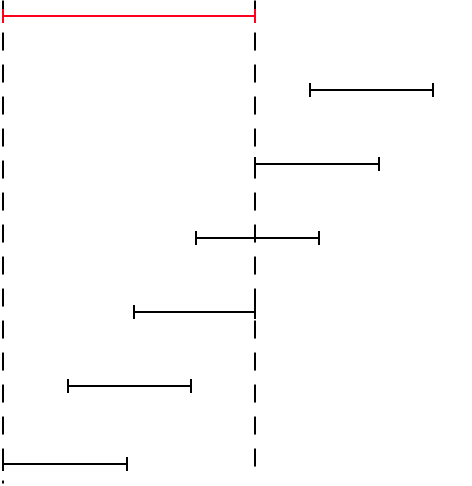
\includegraphics[height=2.02in]{intervals.png}}&\emph{equals} \{=\} &\\
    & &\\
                   &\emph{before} \{\textless\} / \emph{after} \{\textgreater\} & $\langle L \rangle$ / $\langle \overline{L} \rangle$ \emph{(Later)}\\
    & &\\
                   &\emph{meets} \{\emph{m}\} / \emph{met-by} \{\emph{mi}\} &$\langle A \rangle$ / $\langle \overline{A} \rangle$ \emph{(After)}\\
    & &\\
    &\emph{overlaps} \{\emph{o}\} / \emph{overlapped-by} \{\emph{oi}\} &$\langle O \rangle$ / $\langle \overline{O} \rangle$ \emph{(Overlaps)}\\
    & &\\
    &\emph{finished-by} \{\emph{fi}\} / \emph{finishes} \{\emph{f}\} &$\langle E \rangle$ / $\langle \overline{E} \rangle$ \emph{(Ends)}\\
    & &\\
    &\emph{contains} \{\emph{di}\} / \emph{during} \{\emph{d}\} &$\langle D \rangle$ / $\langle \overline{D} \rangle$ \emph{(During)}\\
    & &\\
    &\emph{started-by} \{\emph{si}\} / \emph{starts} \{\emph{s}\} &$\langle B \rangle$ / $\langle \overline{B} \rangle$ \emph{(Begins)}
  \end{tabular}
\end{table}
\subsubsection{Propp Example with Punch and Judy}
In this example, we combine Halpern and Shoham's temporal operators with the possibility ($\Diamond$) and necessity ($\Box$) operators of modal logic. We follow the convention of writing possibility operators inside angle brackets: $\langle \, \rangle$ and necessity operators within square brackets: $[ \, ]$.

This example shows the ``sausages'' scene described in section \ref{sec:pjexample}, consisting of a set of situations $S$, containing Propp story functions $P$. The interval temporal logic operators used in this example are the set $T$. Figure \ref{fig:operators} shows the modal operators we use. $A, B$ and $C$ in formula \ref{eq:story} are variables that represent the characters and objects that appear in the story.
\begin{figure}[!t]
\begin{align}
    S &= \{S_0, S_1, S_2, S_{3a}, S_{3a_1}, S_4, S_{3b}, S_{3b_1}, S_4, S_5\}\\
    P &= \{\mathtt{interdiction(A, B, C), absentation(A), struggle(A, B),}\nonumber\\
  &\qquad\qquad\mathtt{victory(A), villainy(A, B), violation(A, B), return(A)}\}\label{eq:story}\\
  T &= \{D, \overline{D}, O, \overline{O}, A, \overline{A}, B, \overline{B}, L, \overline{L}, E, \overline{E}\}
\end{align}
\caption{Modal operators}\label{fig:operators}
\end{figure}
Hybrid logics allow worlds, time intervals, to be named. The hybrid logic nominal operator allows specific times to be uniquely referenced, allowing a logic to talk about specific states such as $S_0..S_5$. The nominal proposition is true of one specific time interval such that any two worlds with the same name represent co-extensive intervals of time. Anything true of one is true of the other.
We also make use of a nominal modal operator so that it is possible to make assertions about these named worlds, ``It is necessary that in state $S_1$ Joey absents himself.'' This technique enables us to associate story functions with specific, named intervals.
We use hybrid logic to identify nodes using the \emph{nominal} operator, shown as $@$. The nominal operator adds the capability of referring to possible worlds in formulas. In this way, each possible state of a system can be labelled and referenced from other states. As seen in figure \ref{fig:lotrec}, each nominal node must have its own name as a relation leading back to the root node, in order to be linked to and referred from the other nodes.
We can combine this with the Interval Temporal Logic to make statements such as ``An absentation starts with state $@S_1$ and ends with state $@S_5$.'' (formula \ref{eq:absentation}).
Figure \ref{fig:situations} describes the full sausages scene from Punch and Judy using the time intervals shown in figure \ref{fig:durations}.
\begin{figure}[!t]
  \centering
    \centerline{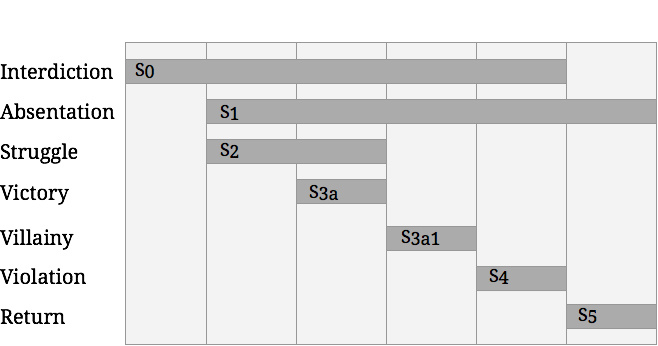
\includegraphics[width=0.9\textwidth]{durations.png}}
  \caption{Timings of the story functions in the sausages scene}\label{fig:durations}
\begin{align}
  &S_{0} \land \mathit{interdiction(Joey, Punch, Sausages)} \land\nonumber\\
  &\qquad\qquad\qquad\qquad\qquad\langle B \rangle @S_{1} \land \langle E \rangle @S_{4} \land \langle A \rangle @S_{5}\label{eq:interdiction}\\
  &[@S_{1}] \mathit{absentation(Joey)} \land \langle A \rangle @S_{2}\label{eq:absentation}\\
  &[@S_{2}] \mathit{struggle(Punch, Crocodile)} \land \langle E \rangle (@S_{3a} \lor @S_{3b})\label{eq:struggle}\\
  &[@S_{3a}] \mathit{victory(Crocodile)} \land \langle A \rangle @S_{3a_1}\\
  &[@S_{3a_1}] \mathit{villainy(Crocodile, Sausages)} \land \langle E \rangle @S_{4}\\
  &[@S_{3b}] \mathit{victory(Punch)} \land \langle A \rangle @S_{3b_1}\\
  &[@S_{3b_1}] \mathit{villainy(Punch, Sausages)} \land \langle E \rangle @S_{4}\\
  &[@S_{4}] \mathit{violation(Punch, Sausages)}\\
  &[@S_{5}] \mathit{return(Joey)}
\end{align}
\caption{Sausages scene with nominals and Interval Temporal Logic}\label{fig:situations}
\end{figure}

One notable feature of this approach is that it enables the building of reusable story components. For example, we have said that an interdiction must begin with an absentation and ends with a violation (formula \ref{eq:interdiction}). This pattern can be reused in different stories, or several times in the same story. Additionally, it allows for the abstraction and combination of story components in a more expressive way than Propp's original story functions. This is because Propp only describes narrative events at one level of abstraction. For example, he describes stories as a series of events containing an interdiction followed by an absentation, followed by a violation. But there is no mechanism for combining these three functions into a higher-level component (which could be called ``Don't do that, or else!'', for example). Our approach makes such abstraction and recombination possible.

\section{Describing Punch and Judy with Kripke Structures}\label{sec:kripke}
\begin{figure}[!t]
  \centering
    \centerline{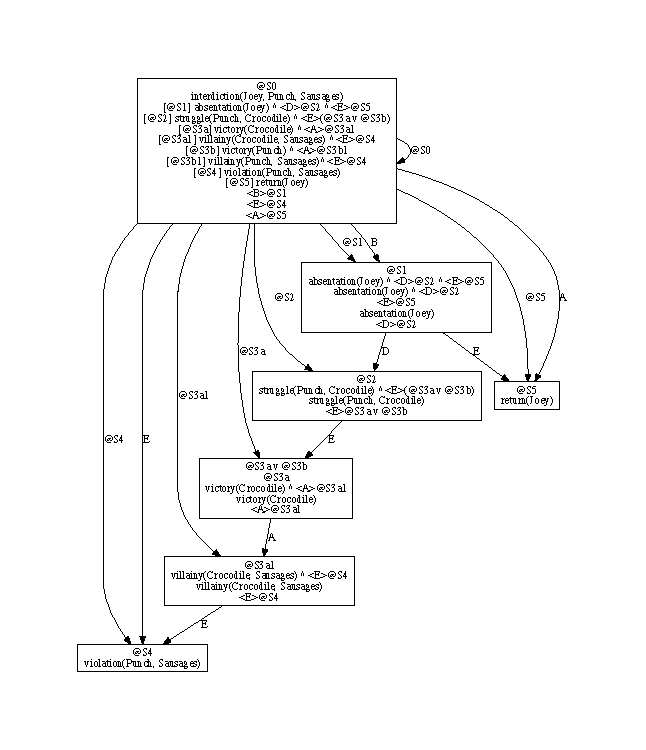
\includegraphics[width=0.9\textwidth]{crocmodel.pdf}}
  \caption{One model from the sausages scene in LoTREC}\label{fig:lotrec}
\end{figure}

We use Kripke structures \cite{kripke1963semantical} as a method of interpreting the combination of modal logic with Interval Temporal Logic. A Kripke structure is a graph, the nodes of which represent a possible world consisting of a set of assertions, and the edges of which are the accessibility relations between worlds.

\subsubsection{LoTREC}
% Read the book
In order to build and visualise the Kripke structures, we use LoTREC \cite{del2001lotrec}, a generic tableaux prover for modal and description logics. It allows the user to build up Kripke models using a domain specific language and display those models in the form of a graph diagram.
LoTREC uses the tableau method for model checking. This method checks whether or not its input is satisfiable by attempting to build a model for it. If the model construction fails, then the input is unsatisfiable.
Building models in LoTREC consists of defining \emph{connectors}, \emph{rules} and \emph{strategies}. Connectors are the logical operators used in formulas, rules are the instructions LoTREC needs to expand them into new nodes and edges and strategies are ways of combining rules in order to form models.
LoTREC takes an initial set of formulas as input and expands each formula into its components. These formulas are input using a simple prefix notation domain specific language consisting of operators and arguments, described in the LoTREC instruction book \emph{Kripke's Worlds} \cite{gasquet2013kripke}.
In the expansion, if a $[\,]$ (necessary) operator is encountered, then the formulas that serve as its argument are propagated across to all subsequent nodes. In the case of a $\langle \, \rangle$ (possibility) operator, a new node (possible world) is created containing its arguments. In both cases, binary operators can be used where one argument is located inside the square or angle brackets. In these cases, the argument inside the brackets is the accessibility relation, and is used to label the edges leading to the subsequent nodes.
In the case of a disjunction ($\lor$) operator, the current model is copied in its entirety and extended with one of the operator's arguments. The other argument is added onto the current model. This is an important way of creating alternative routes through the narrative, all of which can be checked for consistency.

\paragraph{The Sausages Scene in LoTREC}
The narrative is captured as a system of interval temporal logic assertions over story functions. The  assertions are interpreted using a tableaux reasoner by unpacking them to form a Kripke structure.
Using the initial formulas from figure \ref{fig:situations} as input, figure \ref{fig:lotrec} shows the model for the case where Punch wins the fight with the Crocodile. One other model exists in this scenario, in which the Crocodile is instead the victor.

The example in figure \ref{fig:lotrec} describes the fabula of a branching story, where either Punch or the Crocodile may win the fight for the sausages. This corresponds to the disjunction in figure \ref{fig:situations}, formula \ref{eq:struggle}. This leads to the creation of two models: the one in which the Crocodile wins and then goes on to eat the sausages (situation $@S_{3a}$), and the one in which Punch wins (situation $@S_{3b}$).
Using a breadth first strategy like LoTREC we would build all models simultaneously. This enables them to be checked for internal consistency, eliminating potentially impossible temporal arrangements. For example, no interval may come after or later than itself.

The first node contains the logical description of the story, which is then unpacked into subsequent nodes. It starts with the initial situation, $S_0$, which contains an interdiction: $\mathit{interdiction(Joey, Punch, Sausages)}$, where Joey tells Punch to look after the sausages. The other situations, $S_1$ to $S_5$ are listed using the necessity operator, with their accessibility relations being each situation's nominal operator (such as $@S_1$). This means that these situations are all created as new nodes, linked to the root node using their nominal accessibility relation, and so can be referred to later using the nominal operator. In this way, situations can refer to other situations.

For example, in Propp's formalism, an interdiction must begin with the absentation of a character and end with the interdiction's violation. For this reason, the initial situation is connected to $@S_1$, ($\mathit{absentation(Joey)}$), with the $\langle B \rangle$ (begins) accessibility relation and to $@S_4$, ($\mathit{violation(Punch, Sausages)}$), with the $\langle E \rangle$ (ends) accessibility relation. As other situations are unpacked into nodes, they are linked to other situations in the same way. An example of this is shown in $S_1$, the absentation, which must end with Joey's return, $S_5$, and during which a struggle must occur ($S_2$). As the formulas inside $S_1$ are unpacked, $S_1$ is linked to the other situations with the appropriate temporal accessibility relations. This is all made possible with the hybrid logic, which allows nodes to be referred to by name and linked to.

By describing situations that are linked together with temporal relations, we can build narratives and check them as we go. If a narrative is inconsistent in some way (by stating that a character is both dead and alive, for example), then the model will be unsatisfiable. This is useful for ensuring the construction of consistent narratives.

Additionally, every time a story has the possibility of branching off, the model for each new branch can be checked to see if it is viable in the narrative world. This means that rather than relying on an author to write out each branch of a story, they can be generated automatically from a story description and checked for inconsistencies.

As mentioned previously, the combination of Interval Temporal Logic and a narrative formalism such as Propp's allows us to create abstracted story components. For example, we have described the interdiction as being started by an absentation and ended with a violation. This pattern can be called the ``interdiction pattern'', and so can be easily reused in other narratives.

The use of LoTREC has shown the utility of being able to visualise a branching narrative in its entirety. This suggests that our method enables the visual authoring of interactive narratives by non-technical creators. Rather than having to type in computer code, or logical formulas, a visual tool could be developed to create logically consistent narrative worlds.

This approach for describing narrative has many potential real-world uses. One obvious use would be for computer game narratives, but it could also be used to describe a repeatable training scenario, and the possible choices available to a user at any point during the simulation.

\subsection{Deontic Logic and Norms}

\section{Norms and Institutions}
\label{sec:norms-and-institutions}

An institution describes a set of `social' norms describing the permitted and obliged behaviour of interacting agents. Noriega's `Fish Market' thesis~\cite{noriega1999agent} describe how an institutional model can be used to regiment the actions of agents in a fish market auction. Several~\cite{artikis2009specifying,fornara2007agent,cardoso2007institutional} extend this idea to build systems where institutions actively regulate the actions of agents, while still allowing them to decide what to do. We build on the work of Cliffe et al.~\cite{cliffe2007specifying} and Lee et al.~\cite{lee2013decoupling} to adapt it for the world of narrative, using an institutional model to describe the story world of Punch and Judy in terms of Propp's story moves and character roles, through which the actors acquire powers and permissions appropriate to the character and the story function in which they are participating.

Institutional models use concepts from deontic logic to provide obligations and permissions that act on interacting agents in an environment. By combining this approach with Propp's concepts of \emph{roles} and \emph{story moves}, we describe a Propp-style formalism of Punch and Judy in terms of what agents are \emph{obliged} and \emph{permitted} to do at certain points in the story.

For example, in one Punch and Judy scene, a policeman enters the stage and attempts to apprehend Punch. According to the rules of the Punch and Judy world, Punch has an obligation to kill the policeman by the end of the scene (as this is what the audience expects to happen, having seen other Punch and Judy shows). The policeman has an obligation to try his best to catch Punch. Both agents have permission to be on the stage during the scene. The policeman only has permission to chase Punch if he can see him (Punch is obliged to hide from him at the start of the scene).

The permissions an agent has, on the one hand, constrain the choices of actions available to them at any given moment. Obligations, on the other hand, affect the goals of an agent. Whether or not an agent actively tries to fulfil an obligation depends on their emotional state.

\subsection{Institution example}
To illustrate the application of institutional modelling, we here continue the `sausages and crocodile' scene example from section~\ref{sec:pjexample}, taking the Propp story functions and describing them in an institutional model.  We define our institution in terms of \emph{fluents}, \emph{events}, \emph{powers}, \emph{permissions} and \emph{obligations}, following~\cite{cliffe2007specifying}, to which the interested reader is referred for the full details of the formal model, including the generate ($\cal G$) and consequence ($\cal C$) relations, which are only described here in sufficient depth for the model being presented.

\subsubsection{Fluents}
These are properties that may or may not hold true at some instant in time, and that change over the course of time. \emph{Institutional events} are able to \emph{initiate} or \emph{terminate} fluents at points in time. A fluent could describe whether a character is currently on stage, the scene of the story that is currently being acted out, or whether or not the character is happy at that moment in time.
Domain fluents ($\mathcal{D}$) describe domain-specific properties that can hold at a certain point in time. In the Punch and Judy domain, these can be whether or not an agent is on stage, or their role in the narrative: % (equation~\ref{eq:domain}).
\begin{align*}
   \mathcal{D} &= \left\{\mathtt{onstage, hero, villain, victim, donor, item}\right\} %\label{eq:domain}
\end{align*}

Institutional fluents consist of (institutional) \emph{powers}, \emph{permissions} and \emph{obligations}.
% check your facts on this one
An \textbf{institutional power} ($\mathcal{W}$) describes whether or not an external event has the authority to generate a meaningful institutional event. Taking an example from Propp's formalism, an \emph{absentation\/} event can only be generated by an external event brought about by a \emph{donor\/} character (such as their leaving the stage). Therefore, any characters other than the donor character would not have the institutional power to generate an \emph{absentation\/} institutional event when they leave the stage.
The possible empowerments (institutional events) from Propp used in Punch and Judy are:
\begin{align*}
  \mathcal{W} =&\left\{\mathtt{pow(introduction), pow(interdiction), pow(give),}\right.\\ %\nonumber\\
               &\left. {} \mathtt{pow(absentation), pow(violation), pow(return)}\right\} %\label{eq:power}
\end{align*}

\subsubsection{Permissions} ($\mathcal{P}$) are associated with external actions that agents are permitted to do at a certain instant in time. These can be thought of as the set of \emph{socially permitted\/} actions available to an agent. While it is possible for an agent to perform other actions, societal norms usually discourage them from doing so.
% PJ examples
For example, it would not make sense in the world of Punch and Judy if Punch were to give the sausages to the Policeman. It is always Joey who gives the sausages to Punch. Also, it would be strange if Joey were to do this in the middle of a scene where Punch and Judy are arguing. We make sure agents' actions are governed so as to allow them only a certain subset of permitted actions at any one time. The set of permission fluents is:
\begin{align*}
\mathcal{P} =& \left\{\mathtt{perm(leavestage), perm(enterstage), perm(die), perm(kill),}\right.\nonumber\\
             &\left. {} \mathtt{perm(hit), perm(give), perm(fight)}\right\} %\label{eq:perm}
\end{align*}

\subsubsection{Obligations} ($\mathcal{O}$) are institutional facts that contain actions agents \emph{should} do before a certain deadline. If the action is not performed in time, a \emph{violation event} is triggered, which may result in a penalty being incurred. While an agent may be obliged to perform an action, it is entirely their choice whether or not they actually do so. They must weigh up whether or not pursuing other courses of action is worth accepting the penalty that an unfulfilled obligation brings.

% replace with sausages obligation
Anybody who has seen a Punch and Judy show knows that at some point Joey tells Punch to guard some sausages, before disappearing offstage. Joey's departure is modelled in the institution as the \emph{absentation\/} event. It could also be said that Joey has an obligation to leave the stage as part of the \emph{absentation} event, otherwise the story function is violated. This can be described in the institution as:
\begin{align*}
  \mathcal{O} =& \left\{\text{obl}(\mathtt{leavestage, absentation, viol(absentation)})\right\}%\label{eq:obl}
\end{align*}
The first argument is the external event that must be triggered according to the obligation, the second argument is the institutional deadline event, and the third argument is the violation event which is triggered if the obligation is not fulfilled before the deadline. 

\subsubsection{Events}
% actually 3 kinds, including violation events
Cliffe's model specifies three types of \textbf{event}: \emph{external events} (or `observed events', $\mathcal{E}_{obs}$), \emph{institutional events} ($\mathcal{E}_{instevent}$) and \emph{violation events} ($\mathcal{E}_{viol}$). Examples of each are given in Figure~\ref{fig:events}.
\emph{External events} are observed to happen in the agents' environment, which can \emph{generate} \emph{institutional events} which occur only within the institional model, leading to the \emph{initiation} or \emph{termination} of (domain) fluents, permissions, obligations or institutional powers.
An external event could be an agent leaving the stage, an agent hitting another, or an agent dying. Internal events include narrative events such as scene changes, or the triggering of Propp story functions such as \emph{absentation} or \emph{interdiction} (described in section~\ref{sec:propp}). \emph{Violation} is the name of a Propp story function, and is included as an internal event, although it has no relation to the violation events of an institution.
Violation events occur when an agent has failed to fulfil an obligation before the specified deadline. These can be implemented in the form of a penalty, by decreasing an agent's health, for example.

\begin{figure}[!t]
\begin{align}
  \mathcal{E}_{obs} =& \left\{\mathtt{startshow, leavestage, enterstage, die, give,}\right.\nonumber\\
  &\left. {} \mathtt{harmed, hit, fight, kill, escape}\right\}\label{eq:eobs}\\
  \mathcal{E}_{instevent} =& \left\{\mathtt{introduction, interdiction, receipt, absentation,}\right.\nonumber\\
                         &\left. {} \mathtt{violation, return, struggle, defeat, complicity,}\right.\nonumber\\
                         &\left. {} \mathtt{victory, escape}\right\}\label{eq:einst}\\
  \mathcal{E}_{viol} =& \left\{\mathtt{viol(introduction), viol(interdiction), viol(receipt),}\right.\nonumber\\
 &\left. {} \mathtt{viol(absentation), viol(violation), viol(return),}\right.\nonumber\\
 &\left. {} \mathtt{viol(struggle), viol(defeat), viol(complicity)}\right.\nonumber\\
 &\left. {} \mathtt{viol(victory), viol(escape)}\right\}\label{eq:viol}
\end{align}
\caption{External, institutional and violation events for Punch and Judy} \label{fig:events}
\end{figure}

% internal and external

\subsubsection{Event Generation and Consequences}
An \textbf{event generation} function, $\mathcal{G}$, describes how events
($\mathcal{E}$, usually external, but can also be internal) %\mnote{Added $\mathcal{E}$ explanation here}
can generate other (usually institutional) events, conditional upon the current institutional state ($\cal X$). This is the counts-as relation.  For example, if an agent leaves the stage while the \emph{interdiction} event holds, they trigger the \emph{leavestage} event. This combination generates the \emph{absentation} institutional event (rule~\ref{eq:absentation}). Further examples appear in figure~\ref{fig:gen}.

Event generation functions follow a $\langle \mathtt{preconditions} \rangle \rightarrow \{\mathtt{postconditions}\}$ format. The preconditions consist of a set of fluents that hold at that time, along with an event to have occurred. The postconditions are the events that are generated. The generation functions are used to generate internal, institutional events from external events.

Consider the Punch and Judy scenario described in section~\ref{sec:pjexample}. There are seven institutional events (story functions) that occur during this scene: \emph{interdiction}, \emph{complicity}, \emph{receipt} (from Propp's \emph{receipt of a magical agent}) \emph{absentation}, \emph{violation}, \emph{struggle}, \emph{return}.
These institutional events are all generated by external events. The \emph{interdiction} is generated when Joey tells Punch to protect the sausages. Punch agreeing amounts to \emph{complicity}. Joey \emph{gives} punch the sausages (\emph{receipt}), then leaves the stage (\emph{absentation}). The crocodile eating the sausages is a \emph{violation} of Punch's oath, the agents fight (\emph{struggle}), then Joey enters the stage again (\emph{return}).

It is desirable that these story functions occur in this sequence in order for a satisfying narrative to emerge. Agents may decide to perform actions that diverge from this set of events, but the institution is guiding them towards the most fitting outcome for a \emph{Punch and Judy} world. For this reason, a currently active story function can be the precondition for event generation. For example, the \emph{receipt} event may only be triggered if an agent externally performs a \emph{give} action \textbf{and} if the \emph{complicity} event currently holds (rule~\ref{eq:receipt}).
Examples of event generation function for this scenario, complete with preconditions, are listed in rules~\ref{eq:gfirst}--\ref{eq:glast} (Figure~\ref{fig:gen}).

\begin{figure}[!t]
\abovedisplayskip=0pt
\abovedisplayshortskip=0pt
$\mathcal{G(X, E)}:\left\{\mbox{%
{\begin{minipage}[c]{0.85\textwidth}
% \vspace{-2.1em}\begin{align}
\begin{align}
\langle \emptyset,\mathit{tellprotect}\mathtt{(donor, villain, item)} \rangle%\nonumber\\
             %         &\qquad\qquad\qquad
& \rightarrow \left\{\mathit{interdiction}\right\}\label{eq:gfirst}\\
                      \langle \{\mathit{interdiction}\}, \mathit{agree}\mathtt{(villain)}) \rangle %\nonumber\\
            %          &\qquad\qquad\qquad
& \rightarrow \left\{\mathit{complicity}\right\}\\
                      \langle \emptyset, \mathit{give}\mathtt{(donor, villain, item)}) \rangle %\nonumber\\
        %              &\qquad\qquad\qquad
& \rightarrow \left\{\mathit{receipt}\right\}\label{eq:receipt}\\
                      \langle \{\mathit{interdiction}\}, \mathit{leavestage}(\mathtt{donor}) \rangle %\nonumber\\
              %        &\qquad\qquad\qquad
& \rightarrow \left\{\mathit{absentation}\right\}\label{eq:absentation}\\
                      \langle \{\mathit{interdiction}\}, \mathit{harmed}(\mathtt{item}) \rangle %\nonumber\\
         %             &\qquad\qquad\qquad
& \rightarrow \left\{\mathit{violation}\right\}\\
                      \langle \{\mathit{interdiction, absentation}\},
                      \mathit{enterstage}(\mathtt{donor}) \rangle %\nonumber\\
              %        &\qquad\qquad\qquad
& \rightarrow \left\{\mathit{return}\right\}\\
                      \langle \emptyset, \mathit{hit}(\mathtt{donor, villain}) \rangle %\nonumber\\
%                      &\qquad\qquad\qquad
& \rightarrow \left\{\mathit{struggle}\right\}\label{eq:glast}
\end{align}
\end{minipage}}}\right.$
\caption{Event generation in the sausage scene} \label{fig:gen}
\end{figure}

\textbf{Consequences} consist of fluents, permissions and obligations that are \emph{initiated} ($\mathcal{C}^{\uparrow}$) or \emph{terminated} ($\mathcal{C}^{\downarrow}$) by institutional events. For example, the institutional event \emph{receipt} initiates the donor agent's permission to leave the stage, triggering the \emph{absentation} event (rule~\ref{eq:initgive}). When the \emph{interdiction} event is currently active and a \emph{violation} event occurs, the interdiction event is terminated (\ref{eq:interm}). Rules~\ref{eq:cfirst}--\ref{eq:clast} in Figures~\ref{fig:init} and~\ref{fig:term} describe the initiation and termination of fluents in the Punch and Judy sausages scene detailed in section~\ref{sec:pjexample}.

\begin{figure}[!t]
\abovedisplayskip=0pt
\abovedisplayshortskip=0pt
$\mathcal{C^{\uparrow}(X, E)}:\left\{\mbox{%
\begin{minipage}[c]{0.85\textwidth}
\begin{align}
    \langle \emptyset, \mathtt{interdiction} \rangle %\nonumber\\
                                 % &\qquad\qquad
&\rightarrow \{\text{active}(\mathtt{interdiction}), \nonumber\\&\qquad\text{perm}(\mathtt{give(donor, villain, item)})\}\label{eq:cfirst}\\
                                 \langle \emptyset, \mathtt{receipt} \rangle % \nonumber\\
                                 % &\qquad\qquad
&\rightarrow \{\text{perm}(\mathtt{leavestage(donor)})\}\label{eq:initgive}\\
                                 \langle\{\mathit{active(absentation)}\}, \nonumber\\\mathtt{enterstage(villain)} \rangle %\nonumber\\
                                 %&\qquad\qquad
&\rightarrow \{\text{obl}(\mathtt{eat(villain, sausages),} \nonumber\\&\qquad\qquad\mathtt{return, viol(violation)})\}\label{eq:obl1}\\
                                 \langle\{\mathit{active(interdiction)}\}, \nonumber\\\mathtt{leavestage(donor)} \rangle % \nonumber\\
                                 % &\qquad\qquad
&\rightarrow \{\text{obl}(\mathtt{enterstage(donor),}\nonumber\\&\qquad\qquad\mathtt{eat(villain, sausages),}\nonumber\\&\qquad\qquad\mathtt{viol(return)})\}\label{eq:obl2}\\
                                 \{\mathit{active(interdiction)}\},\nonumber\\ \mathtt{violation} \rangle %\nonumber\\
                                 % &\qquad\qquad
&\rightarrow \{\text{perm}(\mathtt{enterstage(dispatcher)})\}\\
                                 \langle\{\mathit{active(absentation),}\nonumber\\\mathit{active(violation)}\},\nonumber\\ \mathtt{return} \rangle %\nonumber\\
                                 %&\qquad\qquad
&\rightarrow \{\text{perm}(\mathtt{hit(donor, villain)})\}
\end{align}
\end{minipage}}\right.$
\caption{Fluent initiation in the sausage scene} \label{fig:init}
\medskip
\abovedisplayskip=0pt
\abovedisplayshortskip=0pt
$\mathcal{C^{\downarrow} (X, E)}:\left\{\mbox{%
\begin{minipage}[c]{0.85\textwidth}
\begin{align}
\langle \emptyset, \mathtt{interdiction} \rangle %\nonumber\\
                                   %&\qquad\qquad
&\rightarrow \{\text{perm}(\mathtt{give(donor, villain, item)})\}\\
                                   \langle \{\mathit{active(interdiction)}\},\nonumber\\ \mathtt{absentation} \rangle %\nonumber\\
                                   %&\qquad\qquad
&\rightarrow \{\text{perm}(\mathtt{leavestage(donor)})\}\\
                                   \langle \{\mathit{active(interdiction)}\},\nonumber\\ \mathtt{violation} \rangle %\nonumber\\
                                   %&\qquad\qquad
&\rightarrow \{\mathit{active(interdiction)}\}\label{eq:interm}\\
                                   \langle \{\mathit{active(absentation),}\nonumber\\\mathit{ active(violation)}\},\nonumber\\ \mathtt{return} \rangle %\nonumber\\
                                   %&\qquad\qquad
&\rightarrow \{\mathit{active(absentation)}\}\label{eq:clast}
\end{align}
\end{minipage}}\right.$
\caption{Fluent termination in the sausage scene} \label{fig:term}
\end{figure}%\mnote{Added \emph{active(interdiction)} to top of fig. \ref{fig:init}}

\section{Why Use Institutions for Interactive Narrative?}
\label{sec:why-use-institutions}
% Write about character freedom, regimentation vs regulation. Give story
% examples vs using a planner

% tropes
% TODO: explain that tropes are not covered academically, I am attempting to
% make tropes academically respectable
% TODO: make it clear at the start that we are choosing these examples as a way
% to demonstrate tropes ability to create abstractions
% TODO: parental abandonment might need extra characters
% TODO: connect character role (such as Comedic Sociopath) to our emotional model
% TODO: connect our idea of phases with landmarks in plans / knowledge
% representation literature
% do also need to demonstrate adequate knowledge of planners
% TODO: put TropICAL / instal fragments in column in appendix, pull out relevant
% features to describe in the chapter
\chapter{Tropes as Story Components}
\label{cha:tropes}
This chapter describes the foundations of our new formalism for narrative: story
tropes. Though our use of tropes for the description of stories has many
advantages, the main advantage that we will focus on throughout this thesis is
that they provide a means of creating new abstractions from existing tropes. For
more detail on how tropes allow us to do this, please see section~\ref{sec:abstractable}

Though story tropes may be a familiar concept to many outside of the academic
community, they do not appear in the literature in either fields Computer Science or
Narratology at the time of writing. Therefore this chapter contains a thorough
description of what a story trope is, along with several examples.

As previously described in chapter~\ref{cha:introduction}, tropes are
patterns that appear throughout various different media. Once one is familiar
with a trope, it becomes easy to identify its use in any story. Take, for
example, the \emph{Hero's Journey} trope first described in
chapter~\ref{cha:introduction}. It is a template which is repeated so often in
many different media, stories and contexts that it is instantly recognised even
by those that are completely unfamiliar with the concept of tropes.

% Bit about difference between tropes and cliches

In this section we examine the concept of a ``trope'', deconstructing examples
to demonstrate widely-recognised trope patterns, and exploring tropes that
operate at different levels of abstraction within a story. At the end of the
section we identify a formal definition of a trope, and how it fits within the
wider context of a story.

% TODO NUMBER
% TODO list of examples where tropes appear from jurisin paper
% TODO TVtropes screenshot figure
% TODO describe the periodic trope groups
\section{Tropes: a ``Folksonomy'' of Story Components}
The existence of a website called ``TV Tropes''~\citep{tvtropes} makes the discovery of example
tropes very simple. TV Tropes is a wiki for tropes, containing over 27,000
trope descriptions, along with the media that they appear in. For example, the
``The Empire'' trope appears in \emph{Star Wars}, Asimov's \emph{Foundation}
trilogy, the \emph{Hunger Games} books and films, and the \emph{Final Fantasy}
series of games, and a great many more stories in media.


\begin{figure}[!t]
\centerline{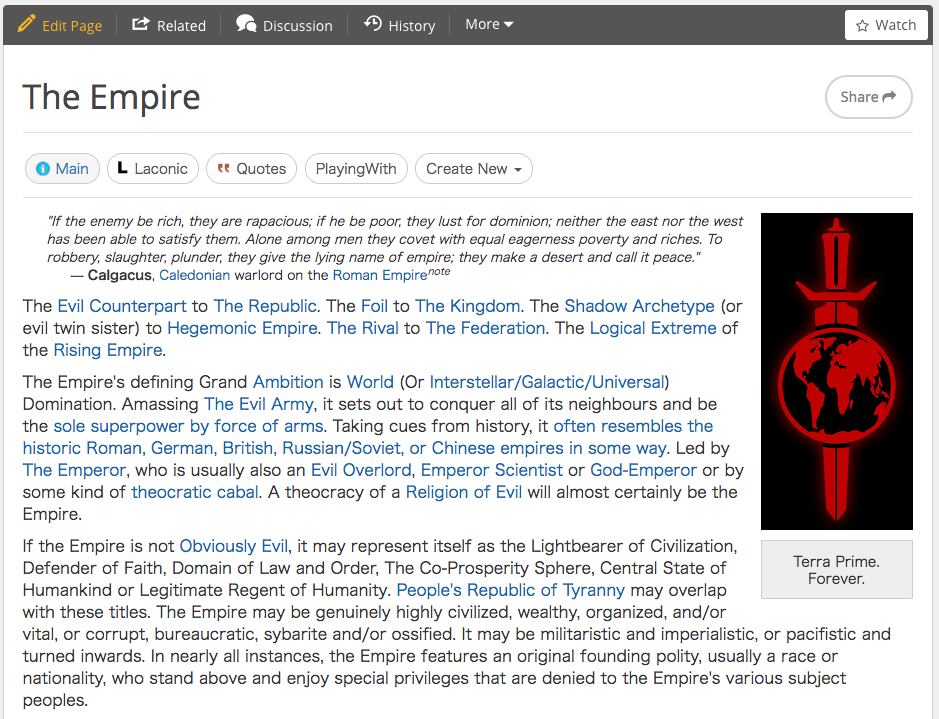
\includegraphics[height=5in]{evilEmpire.png}}
\caption{A screenshot of the ``The Empire'' wiki page from TV Tropes} \label{fig:evil-empire}
\end{figure}

Figure~\ref{fig:evil-empire} shows a screenshot of the ``The Empire'' page on the
website. It clearly shows the description of the trope at the top of the page,
and there are also instances of its use across different media at the bottom.

Tropes can also describe character archetypes. For example, this is how TV
Tropes describes \emph{Anti-Hero} characters:

\begin{quote}
An Archetypal Character who is almost as common in modern fiction as the Ideal Hero, an antihero is a protagonist who has the opposite of most of the traditional attributes of a hero. They may be bewildered, ineffectual, deluded, or merely apathetic. More often an antihero is just an amoral misfit. While heroes are typically conventional, anti-heroes, depending on the circumstances, may be preconventional (in a "good" society), postconventional (if the government is "evil") or even unconventional. Not to be confused with the Villain or the Big Bad, who is the opponent of Heroes (and Anti-Heroes, for that matter).
  \end{quote}

TV Tropes further clarifies that there are even further subdivisions of
Anti-Hero, depending on just how evil or cynical the character is. Batman, for
example, would be a highly cynical Anti-Hero who is nevertheless morally good.

Shakespeare's Macbeth is a character who becomes more and more of an evil Anti-Hero, until he is too morally evil
to still be a Hero and instead becomes a Tragic Villain.

Tropes can be very specific, referring to individual lines of dialogue.
One example is ``We Will Meet Again'':

\begin{quote}
The standard phrase when the villain finds that he has been defeated by the heroes and there is no point in staying around with the immediate Evil Plan foiled.
\end{quote}

Tropes can also be very abstract, referring to particular genres, types of
story, or events in a story that move the action forward. Other than the
previously mentioned ``Hero's Journey'' and ``The Empire'' tropes, another
example could be the ``Hilarity Ensues'' trope:

\begin{quote}
Actions that are dangerous or illegal often lead to injury, arrest, job dismissal, expulsion from school, deportation, or other dire consequences. Thankfully for our fictional friends, both the Rule of Cool and the Rule of Funny keep them safe (the latter more prominently).
\end{quote}

\emph{Metatropes} are tropes about tropes, often intended as a knowing wink to
the trope-savvy audience. One such example is ``Lampshade Hanging'', which TV
Tropes describes as:

\begin{quote}
...the writers' trick of dealing with any element of the story that threatens the audience's Willing Suspension of Disbelief, whether a very implausible plot development, or a particularly blatant use of a trope, by calling attention to it and simply moving on.
\end{quote}

In fact, even if an audience is unaware of the concept of tropes, they may be aware
of the recurring patterns and themes that they describe. This enables
genre-savvy (and especially postmodern) writers to play with the audience's
expectations. Ways to do this with tropes could include \emph{inversion}
(reversing the trope),
\emph{subversion} (making it look like the trope will happen, but then not using
it after all), \emph{parody} (using the trope in an over-the-top, exaggerated
manner) and \emph{deconstruction} (using the trope in a straightforward manner,
but in way which forces the audience to analyse the trope itself).

Take, for example, the well-known ``The Butler Did It'' trope from murder
mystery stories, where the butler of the house is revealed to be the murderer at
the end of the story. TV Trope describes ways that an author could ``play'' with this trope:

\begin{compactitem}
  \item \textbf{Subvert} it: The butler is the prime suspect at the beginning, and is later found innocent.
  \item \textbf{Invert} it: The butler is the victim. Or the butler solved the crime. Or every suspect except the butler was part of the crime.
  \item \textbf{Parody} it: Butlers could learn their trade at butler college where they are taught cleaning, cooking, and murdering.
  \item \textbf{Deconstruct} it: The butler is a revolutionary serial killer, who purposely takes jobs as butlers to murder his rich masters. All the unfortunate implications of class warfare that this suggests are brought up and discussed.
\end{compactitem}

Many other examples of using tropes in this way can be found on the ``Playing
with a Trope'' page of the TV Tropes website~\cite{playing-tropes}.


\begin{figure}[p!]
\centerline{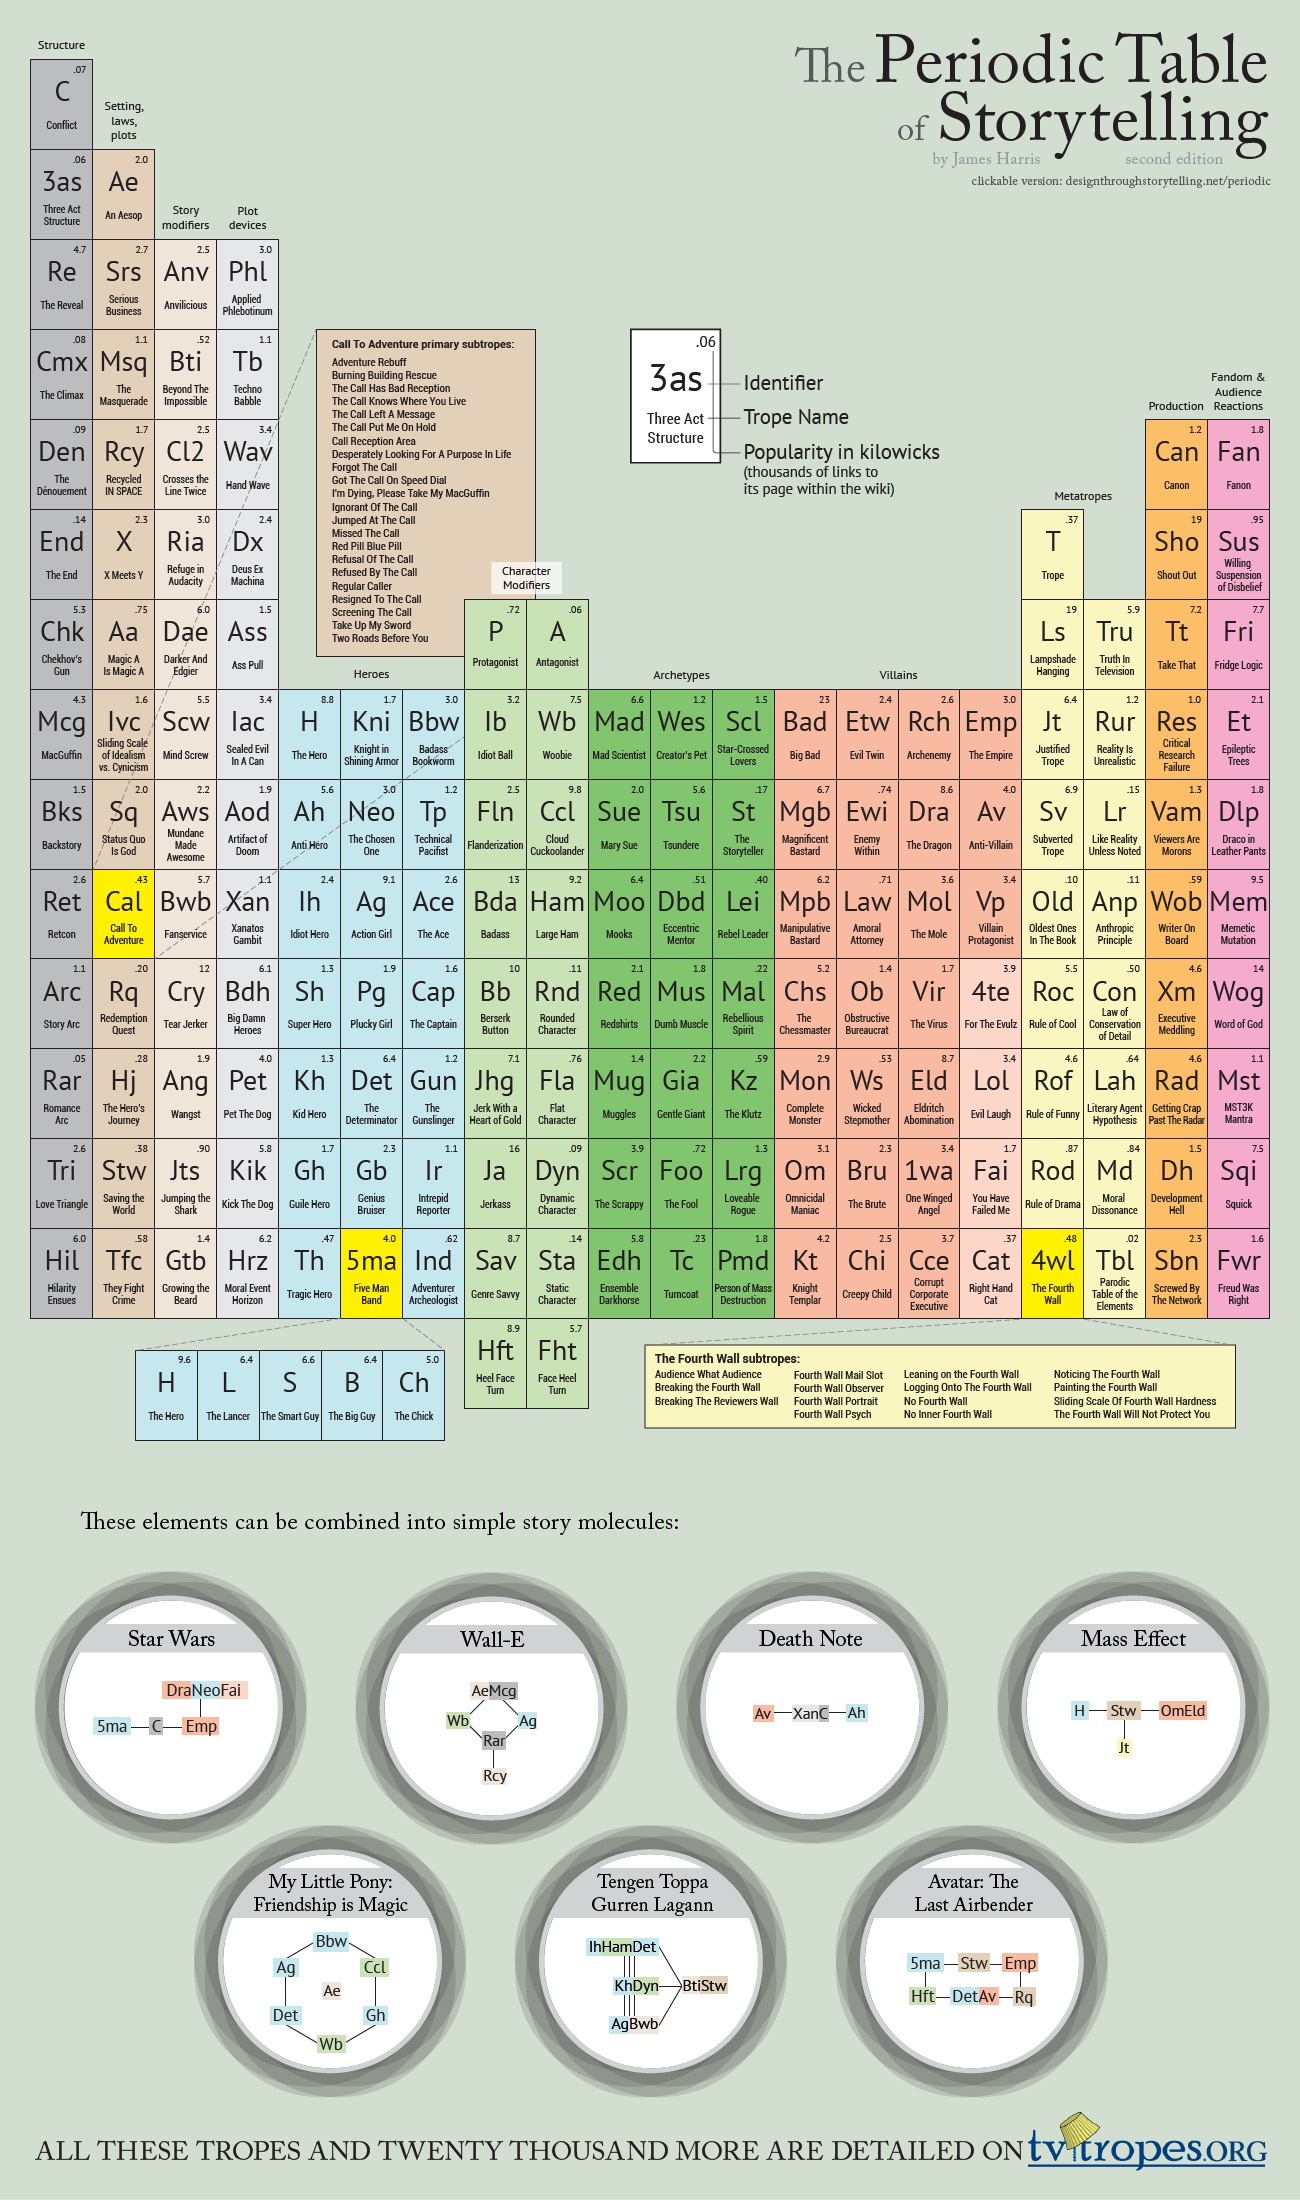
\includegraphics[height=\textheight]{periodicTable.png}}
\caption{The ``Periodic Table of Storytelling'', original by James Harris
  (http://jamesharris.design/periodic/), poster format by Deviant Art user Dawn
  Paladin (http://dawnpaladin.deviantart.com/art/The-Periodic-Table-of-Storytelling-Second-Edition-425816342)} \label{fig:periodic-table}
\end{figure}

A large and highly active community of users and contributors exists around TV
Tropes. In addition to creating content for and curating the content on the
website, they also work to create useful ways to visualise the usage of tropes
in stories. For example, The Periodic Table of
Storytelling~\citep{periodicTableOfStorytelling} is a visualisation of tropes as
``elements'' in the ``molecules'' of a story. The table itself
(fig.~\ref{fig:periodic-table}) arranges the tropes into different ``groups''
according to the part of a story that they operate on. The leftmost groups
describe the story as a whole, describing its \emph{structure} (``Three Act
Structure'', ``MacGuffin'', ``Chekov's Gun''), \emph{story
  modifiers} (``Darker and Edgier'', ``Tear Jerker'', ``Jumping the Shark''),
and \emph{plot devices} (``Hand Wave'', ``Techno Babble'', ``Xanatos Gambit'').
In the centre of the table are different types of character such as
\emph{Heroes} (``Anti Hero'', ``Action Girl'', ``The Gunslinger''),
\emph{Archetypes} (``Mad Scientist'', ``The Fool'', ``Loveable Rogue'') and
\emph{Villains} (``Evil Twin'', ``The Empire'', ``Obstructive Bureaucrat''). The
right third of the table contains self-referential tropes such as
\emph{metatropes} (``Lampshade Hanging'', ``Subverted Trope'', ``The Fourth
wall''), and \emph{fandom and audience reactions} (``Fanon'', ``Fridge Logic'',
``Freud Was Right'').

The story is then visualised as a molecule composed from tropes, linked together as
atoms (shown at the bottom of fig.~\ref{fig:periodic-table}).

This visualisation demonstrates the core idea of our use of tropes as reusable
story components, but the ``molecule'' metaphor is unsuitable for a couple of
reasons. Firstly, linking tropes together as atoms in a molecule does not
communicate the different levels of abstraction at which tropes operate.
Considering that our main purpose for choosing tropes as our method of
describing narrative components, this means that the ``molecule'' metaphor used
by the author does not match our intentions. The
``Hero's Journey'' trope, for example, would describe the narrative arc as a
whole, while the ``Comeuppance'' trope would describe just a single scene in the
story. The metaphor is also not ideal because it presents orthogonal concepts
together in a story with no indication of which part of a narrative they affect.
A ``scoundrel sidekick'' could be linked together with a ``breaking the fourth
wall'' trope, even though one trope relates to a certain character, and the
other may describe a single line of dialogue or action that occurs at a specific
point in the story. 

Also, the arrangement and linking of the tropes in the example molecules is
quite arbitrary. The examples given on the \emph{periodic table} web site form
interesting shapes, but do not follow a consistent logic. In the \emph{Star
  Wars} molecule, for example, the ``Five Man Band'', ``Conflict'' and ``The
Empire'' tropes are linked in a straight line suggesting a linear sequence, but
three further tropes (``The Dragon'', ``The Chosen One'' and ``You Have Failed
Me'') are all linked to the ``The Empire'' trope in the molecule. While ``The
Dragon'' refers to the Death Star in the movie, the ``The Chosen One'' trope is
more closely linked to Luke Skywalker's Hero role. The ``You Have Failed Me''
trope refers to a specific scene where villain Darth Vader punishes an
under performing henchman with choking. It is not clear why the creator decided
to link these specific tropes to the ``The Empire''
trope.

Similarly, in the \emph{GhostBusters} example, the ``Five Man Band'' and ``Mad
Scientist'' tropes appear together in the same ``atom'', which are linked to
``Sealed Evil in a Can'' and ``Hilarity Ensues''. Again, it is not clear why
those particular tropes are arranged together into the same atoms, or why they
are linked together in this way. The most likely explanation is that this
visualisation of the way that tropes link together in a story is not intended as
a serious way to formalise stories, and is merely a ``fun'' example.

Taking this visualisation as inspiration, we develop our concept of tropes as
logical, reusable components for the formal description of stories. Importantly,
we develop a way to nest tropes within other tropes as subtropes as a way to
describe tropes acting at different levels of abstraction.

% TODO rip the whole bit from the lit review? Consider it at least
\section{Why Use Tropes?}
% Write about ability to abstract, give story examples vs Propp
% This is pretty much covered in the lit review

Returning to the shortcomings of existing narrative formalisms we describe in
section~\ref{litrev-discussion}, we now describe how tropes are suitable for use
as a narrative formalism that is able to overcome these limitations.

\subsection{A Means of Abstraction}
\label{sec:abstraction}
Most tropes exist in a hierarchy of tropes, with parent tropes such as the
\emph{Quest} containing child tropes such as \emph{Redemption Quest},
\emph{Sidequest} or a \emph{Quest for Identity}. These child-tropes inherit some
of the characteristics of their parents, but add subtle or major changes. For
example, a \emph{Quest for Identity} follows the \emph{Quest} format, but is
constrained so that the item the hero is questing after is the hero's own
identity. This is a mechanism of \emph{inheritance}, so one can imagine using
such a process to avoid duplication of effort when authoring new tropes by only
expressing how a trope differs from its parent.

\begin{figure}[!t]
\centerline{
\includegraphics[height=1.5in]{freytag.png}}
\caption{Freytag's Pyramid} \label{fig:freytag}
\end{figure}

Another method of abstraction is to express tropes that are contained as parts
of larger tropes. The example we described in section~\ref{litrev-discussion}
describes how the ``Quest'' trope could form just one part of a larger trope
such as the ``Hero's Journey''. Another example of this would be the
\textbf{Three Act Structure} (also known as Freytag's Pyramid) shown in fig.~\ref{fig:freytag}, which describes the shape of a
story in terms of rising and falling levels of drama. This could be split into
five (or perhaps more) sub-tropes:

\begin{compactitem}
  \item \textbf{Exposition}: The setting of the scene, providing any background
    information that is relevant to the story.
  \item \textbf{Rising Action}: A series of event drive the story forward, each
    increasing in dramatic intensity.
  \item \textbf{Climax}: The turning point of the story. Some fateful event
    occurs as a result of the rising action, which could be a battle between the
    hero and the villain, for example.
  \item \textbf{Falling Action}: The consequences of the climax play out, and
    the story shows how the characters are affected.
  \item \textbf{Denouement}: This is the final resolution, where all the ``loose
    ends'' of the story are tied up.
\end{compactitem}

This means that if we already have trope definitions for the ``Exposition'',
``Rising Action'', ``Climax'', ``Falling Action'' and ``Denouement'' parts of a
story, and want to create a ``Three Act Structure'' trope, we can simply express
it in the following way:

\begin{compactitem}
  \item The ``Exposition'' trope happens
  \item Then the ``Rising Action'' trope happens
  \item Then the ``Climax'' trope happens
  \item Then the ``Falling Action'' trope happens
  \item Then the ``Denouement'' trope happens
\end{compactitem}

Returning to the concept of ``story structure'' described in
section~\ref{sec:structure}, we can use the ``subtropes'' we just identified to
describe other ``story shapes'' as defined by Vonnegut. For example, the ``man
in hole'' story shape could be simple described as a rearrangement of the
three-act structure:

\begin{compactitem}
  \item The ``Exposition'' trope happens
  \item Then the ``Falling Action'' trope happens
  \item Then the ``Zenith'' trope happens
  \item Then the ``Rising Action'' trope happens
  \item Then the ``Climax'' trope happens
  \item Then the ``Denouement'' trope happens
\end{compactitem}

Note that we added an additional trope, the ``Zenith'' trope to describe the
lowest point in the story. Otherwise, the rest of the story ``shape'' is easily
described in terms of tropes that we have defined already.

This re-use of existing trope definitions saves us the time and effort of the wasteful duplication of the steps
already described within them. This is why abstraction is such a powerful
and useful concept: it allows us to break down complicated stories into a series
of smaller sub-stories, rather than having to describe the whole thing in one go.

\subsection{Conceptually Simple}\label{sec:tropes-simple}

Most story authors are already familiar with the concept of tropes. In order to
evaluate the suitability of their use for the description of narrative
components, we presented a preliminary version of our trope-based TropICAL programming
language (described in section~\ref{}) for story authoring to the Oxford and London Interactive Fiction meetup group.

After a brief presentation on the concept of tropes and how we intend to use
them to create an authoring system for interactive narrative, participants were
given a questionnaire with the purpose of discovering their familiarity with
tropes, as well as finding out how suitable they thought tropes would be as a
new kind of formalism for narrative components.

There were 18 responses to the questionnaire. The questions and responses were as follows:

\textbf{What's your interest in Interactive Fiction?}
\begin{compactitem}
  \item I'm an author: 5 (27.8\%)
  \item I'm a game developer: 10 (55.6\%)
  \item I write interactive fiction: 5 (27.8\%)
  \item It's my hobby: 6 (33.3\%)
  \item It's my job: 5 (27.8\%)
  \item Other: 2 (11.1\%)
\end{compactitem}
\textbf{What tools do you use to create Interactive Fiction?}
\begin{compactitem}
  \item Inform: 3 (16.7\%)
  \item Twinery: 7 (38.9\%)
  \item Unity or other IDE: 8 (44.4\%)
  \item Pure code: 4 (22.4\%)
  \item I don't create interactive fiction or games with narrative: 3 (16.7\%)
  \item Other: 6 (33.3\%)
\end{compactitem}
\textbf{What kind of narratives are you interested in making?}
\begin{compactitem}
  \item Linear: 2 (11.1\%)
  \item Non-linear: 11 (61.1\%)
  \item I'm not an author: 1 (5.6\%)
  \item Other: 4 (22.2\%)
\end{compactitem}
\textbf{Are you familiar with the idea of ``tropes''?}
\begin{compactitem}
  \item Yes, and I have visited the ``TV Tropes'' website: 15 (83.3\%)
  \item Yes, but I hadn't heard of ``TV Tropes'': 3 (16.7\%)
  \item No: 0 (0\%)
\end{compactitem}
\textbf{How useful do you think tropes are for authoring interactive stories?
  (on a scale of 1 - 5)}
\begin{compactitem}
  \item \textbf{1} (not useful): 0 (0\%)
  \item \textbf{2}: 2 (11.8\%)
  \item \textbf{3}: 9 (52.9\%)
  \item \textbf{4}: 2 (11.8\%)
  \item \textbf{5} (extremely useful): 4 (23.5\%)
\end{compactitem}

The fact that all of the interactive fiction authors and games developers were
already familiar with the concept of tropes demonstrates that they are
conceptually simple enough for non-programmers to understand. Not only that, but
most of them were already familiar with the TV Tropes website. Compare this with
formalisms for narrative components such as Lehnert's Plot
Units~\citep{lehnert1981plot}, which would only be familiar to computer science specialists.

\subsection{A Library of Re-usable Examples}

One of the major strengths of Propp's system~\cite{propp1968morphology} is that
the Morphology is not only a theory: it is also a library of 31 story functions
that can be put together by story authors to create a narrative. The authors
need not create their own story functions, they can simply use the ones that
Propp has already created for them.

Our system shares the same strength due to the fact that the TV Tropes website
serves as our ``library'' of story components. In addition, it grants authors
the flexibility to create their own tropes which are not already listed on the
TV Tropes website.

TropICAL, our domain-specific programming language for trope-oriented story
authoring, makes the authoring of story tropes simple for non-programmer users.
In the same vein as Inform 7~\citep{reed2010creating}, our language uses a
constrained natural language syntax. Further details are described in
section~\ref{sec:tropical}, where we describe the language in detail. In the same manner as a wiki, once a number of authors have contributed tropes,
it will become a useful library of reusable tropes for future authors to use in
their stories.

To summarise: tropes are an ideal model to use for story components, and fulfil
the criteria we laid out in section~\ref{sec:litrev-discussion}: they provide a
\emph{means of abstraction} through subtropes as well as parent and child
tropes, they are \emph{conceptually simple} for authors to learn, given that
most authors are already familiar with them, and they enable us to easily create
a \emph{library of re-usable examples} from the tropes listed on the TV Tropes website.

% \section{Using Tropes with Modal Logic}
% In section~\ref{sec:pjexample}, we described the ``sausages'' scene from
% \emph{Punch and Judy} by combining Propp's story functions with modal operators
% to create Kripke structures to visualise the paths through the scene. In order
% to compare the expressiveness of tropes as a story formalism, this section
% describes the same scene, but instead using tropes in place of Propp functions.

% ACTUALLY DO THIS!

\section{Describing Tropes as Institutions} % 1/2
\label{sec:tropes-as-insts}
Rather than strictly telling our story characters what to do to conform to a
story arc, we govern their behaviours with \emph{social institutions}, as
described in Section~\ref{sec:institutions}. An institution describes a set of `social' norms describing the permitted and obliged behaviour of interacting agents. Noriega's `Fish Market' thesis~\cite{noriega1999agent} describes how an institutional model can be used to regiment the actions of agents in a fish market auction.~\cite{cliffe2007specifying},~\cite{lee2013decoupling} extend this idea to build systems where institutions actively regulate the actions of agents, while still allowing them to decide what to do. Adapting this idea to the world of narrative, we use an institutional model to describe the tropes that occur within a story world.

Institutional models use concepts from deontic logic to provide obligations and permissions that act on interacting agents in an environment. By combining this approach with the idea of tropes, we can create a narrative model in terms of what agents are \emph{obliged} and \emph{permitted} to do at certain points in the story. In this way, the tropes are described as social norms which govern the character agents of a story, where an institution describes the norms that govern a certain trope, and a story is a collection of tropes.

In order to describe story tropes in terms of social norms, we break them down into three components:

\begin{compactenum}
\item characters, which instantiate roles
\item objects, which instantiate types
\item places, which instantiate locations
\end{compactenum}

Characters' actions are described in terms of permissions and obligations. For example, a character in a certain role \emph{may} go to the cinema, or a character \emph{must} buy a ticket before the movie begins, otherwise they will not see it. Note that an obligation (which says that a character \emph{must} do something) can have a deadline (``before the movie begins'') and a consequence (``they will not see the movie''). These are both optional in our system.

Returning to the tropes described in the introduction, we can express them in terms of social norms:

\begin{compactitem}
  \item \textbf{The Hero's Journey}: The hero \emph{must} leave home when they receive the call to adventure. Then the hero \emph{may} kill the villain. Once this is done, the hero \emph{may} return home.
  \item \textbf{The Evil Empire}: The villain has an empire, and \emph{may} kill the hero.
  \item \textbf{MacGuffin}: The hero \emph{must} search for an object. However, the hero \emph{may} find it.
  \item \textbf{Chekhov's Gun}: If a weapon appears in the beginning, it \emph{must} be used before the end of the story.
\end{compactitem}

Describing tropes in terms of permissions and obligations is enough for us to be able to specify them as social norms, but also we need to be able to determine which norms hold at any point of a story. For this, we use an \emph{Answer Set Programming} (ASP) approach to describe our tropes in order to use an answer-set solver. We do this with the aid of \emph{InstAL}~\citep{cliffe2007specifying}, the Institution Action Language, a language for describing social institutions, which compiles to AnsProlog. This allows us to use trope models and an ASP solver to determine which norms hold after agent or player actions have occurred in the story world.

In InstAL, external events trigger institutional (internal) events. External events are the actions of the character agents in their environment. For example, an agent playing the role of Luke Skywalker in a Star Wars game may pick up a Lightsaber. Since Luke Skywalker is a hero character, and a Lightsaber is a type of weapon, this would trigger an institutional event where a hero has picked up a weapon. Institutional events initiate and terminate fluents inside the institution, which may describe the institutional state, and which permissions and obligations currently hold. So when Luke Skywalker picks up a Lightsaber, the institutional event could initiate his permission to use the weapon, or an obligation to go to the land of adventure.
For more details on InstAL, social institutions, and the formalism in figures~\ref{fig:events} and~\ref{fig:term}, refer to~\citep{cliffe2007specifying}.

Figure~\ref{fig:events} lists some external ($\mathcal{E}_{external}$) and institutional (internal, $\mathcal{E}_{internal}$) events for the \emph{Hero's Journey} trope. A wide range of external events such as \emph{go}, \emph{meet}, \emph{kill}, \emph{escape} generate the \emph{intHerosJourney} internal event, but only if the external event meets certain criteria. These criteria could be whether or not an agent fulfils a certain role, for example. Figure~\ref{fig:gen} shows examples of such internal event generation ($\mathcal{G}$). In the first example (rule~\ref{eq:tatooine}), the \emph{intHerosJourney} event is generated when Luke Skywalker goes to Tatooine, but only if Luke has the role of \emph{hero}, and Tatooine's location is \emph{home}.
Figure~\ref{fig:init} shows how internal events initiate ($\mathcal{C^{\uparrow}}$) fluents and norms (permissions and obligations) in a trope. Because the \emph{Hero's Journey} trope has several stages, this example only shows the first two phases of the trope (this is explained further in the ``Sequencing'' part of the ``TropICAL: a DSL for Tropes'' section). Rule~\ref{eq:phaseb} shows how the \emph{intHerosJourney} internal event initiates the hero's permission to kill the villain, an obligation for the hero to go to the Land of Adventure before the villain kills the victim, and the next phase (phase C) of the \emph{Hero's Journey} trope. These fluents are only initiated if the \emph{intHerosJourney} internal event happens while the trope is in phase B (when \emph{phase(herosJourney, phaseB)} holds), however.
Fluent termination ($\mathcal{C^{\downarrow}}$) works in a similar manner to initiation, with permissions and obligations for previous trope phases being terminated once the next phase of a trope has been entered. Examples for the first two phases of the \emph{Hero's Journey} trope are shown in figure~\ref{fig:term}.

While InstAL allows us to express tropes as social institutions, it would be difficult to use for non-programmers who are unfamiliar with logic programming paradigms. In order for story authors to be able to create their own tropes, a much more user-friendly language is needed. This is the motivation for TropICAL, the domain specific language we describe in the next section.

\begin{figure}[!t]\small
\begin{align}
  \mathcal{E}_{external} = & \left\{\begin{array}{c}
\mathtt{go(Agent, Place)},\\
\mathtt{meet(Agent, Agent)},\\
\mathtt{kill(Agent, Agent)}\\
\mathtt{escape(Agent)}
\end{array}
\right\}\label{eq:eobs}\\
  \mathcal{E}_{internal} = &\left\{\begin{array}{l}
\mathtt{intHerosJourney(Agent,}\\
\;\;\mathtt{Agent, Agent, Place, Place)}
\end{array}\right\}
\label{eq:einst}
\end{align}
\caption{External and institutional events ($\mathcal{E}$) for the \emph{Hero's Journey} trope} \label{fig:events}
\end{figure}

\begin{figure*}[!t]
\small
%------------------------------------------------------------------------
The generation relation $\mathcal{G}$ for trope state $\mathcal{X}$ and external event $\mathcal{E}$ in the \emph{Hero's Journey} trope:\\ 
$\mathcal{G(X, E)}:\left\{\mbox{%
\begin{minipage}[c]{0.85\textwidth}
\begin{align}
\begin{array}{r}
\langle \{\mathit{role(lukeSkywalker, hero)},\\
\mathit{location(tatooine, home)}\},\\
\mathit{go}\mathtt{(lukeSkywalker, tatooine)} \rangle
\end{array}
&\rightarrow
\begin{array}{l}
\{\mathit{intHerosJourney}\mathtt{(lukeSkywalker,}\\\;\;\;\;\mathtt{R, S, tatooine, T)}\}
\end{array}\label{eq:tatooine}\\
\begin{array}{r}
                                 \langle \{\mathit{role(lukeSkywalker, hero)},\\
  \mathit{role(obiWan, dispatcher)}\},\\
\mathit{meet}\mathtt{(lukeSkywalker, obiWan)} \rangle
\end{array}
&\rightarrow
\begin{array}{l}
\{\mathit{intHerosJourney}\mathtt{(lukeSkywalker,}\\\;\;\;\;\mathtt{obiWan, R, S, T)}\}
\end{array}\label{eq:hsnth}
\end{align}
\end{minipage}
}\right.$\smallskip

%------------------------------------------------------------------------
The fluent initiation relation $\mathcal{C^{\uparrow}}$ for trope state $\mathcal{X}$ and internal event $\mathcal{E}$ in the \emph{Hero's Journey} trope:\\
$\mathcal{C^{\uparrow}(X, E)}:\left\{\mbox{%
\begin{minipage}[c]{0.85\textwidth}
\begin{align}
\begin{array}{r}
                                 \langle \{\mathit{phase(herosJourney, phaseA)}\},\\
  \mathit{intHerosJourney(hero, dispatcher, villain},\\
\mathit{home, landOfAdventure)}\} \rangle
\end{array}
&\rightarrow
\left\{\begin{array}{l}
\text{perm}(\mathtt{meet(hero, dispatcher)})\\
\text{phase}(\mathtt{herosJourney, phaseB})
\end{array}\right\}\label{eq:cfirst}\\
\begin{array}{r}
                                 \langle\{\mathit{phase(herosJourney, phaseB)},\\
  \mathit{intHerosJourney(hero, dispatcher, villain},\\ \mathit{home, landOfAdventure)}\} \rangle\\
  \end{array}
&\rightarrow \left\{
\begin{array}{l}
  \text{perm}(\mathtt{kill(hero, villain)}) \\
\text{obl}(\mathtt{go(hero, landOfAdventure),} \\
\mathtt{kill(villain, victim)},\\
\mathtt{viol(story, end)})\\
\text{phase}(\mathtt{herosJourney, phaseC})
\end{array}
\right\}\label{eq:phaseb}
\end{align}
\end{minipage}
}\right.$\smallskip

%------------------------------------------------------------------------

The fluent termination relation $\mathcal{C^{\downarrow}}$ for trope state $\mathcal{X}$ and internal event $\mathcal{E}$ in the \emph{Hero's Journey} trope:\\
$\mathcal{C^{\downarrow} (X, E)}:\left\{\mbox{%
\begin{minipage}[c]{0.85\textwidth}
\begin{align}
\begin{array}{r}
                                 \langle \{\mathit{phase(herosJourney, phaseA)}\},\\
  \mathit{intHerosJourney(hero, dispatcher, villain},\\ \mathit{home, landOfAdventure)}\} \rangle
  \end{array}
&\rightarrow \left\{
\begin{array}{l}\text{perm}(\mathtt{go(hero, home)}),\\
\text{phase}(\mathtt{herosJourney, phaseA})
\end{array}
\right\}\label{eq:crt}\\
\begin{array}{r}
                                 \langle\{\mathit{phase(herosJourney, phaseB)},\\
  \mathit{intHerosJourney(hero, dispatcher, villain},\\ \mathit{home, landOfAdventure)}\} \rangle
  \end{array}
&\rightarrow \left\{
\begin{array}{l}
\text{perm}(\mathtt{meet(hero, dispatcher)})\\
\text{phase}(\mathtt{herosJourney, phaseB})
\end{array}
\right\}\label{eq:crst}
\end{align}
\end{minipage}
}\right.$
\caption{Generation events, and fluent initation and termination for the Hero's Journey trope}
\label{fig:gen}
\label{fig:init}
\label{fig:term}
\end{figure*}

\section{Punch and Judy as Tropes}
\label{sec:punchjudy-tropes}
In section~\ref{sec:pjexample}, we describe the \emph{sausages} scene of Punch
and Judy in terms of Propp's story functions. We begin this section in the same
way, by building up a scene description in terms of tropes. Then, as in
section~\ref{sec:pjexample-insts}, we create an institution out of the scene we
have described with our formalism. 

On the TV Tropes page for Punch and Judy, it lists the following tropes (quoted
directly from the site):

\begin{compactitem}
  \item \textbf{Amusing Injuries}: People are often beaten up.
  \item \textbf{Audience Participation}: The children are expected to reply to Mr. Punch's Catch Phrase, "That's the way to do it" with a shout of "Oh no, it isn't!"
  \item \textbf{Black Comedy}: So black that many modern versions are often heavily censored compared to more historical stagings.
  \item \textbf{Catch Phrase}: ``That's the way to do it!'', ``HE'S BEHIND
    YOU!'', etc.
  \item \textbf{Comedic Sociopath}: Mr. Punch
  \item \textbf{Commedia dell'Arte}: Punch is based on the \emph{Pulcinella} character.
  \item \textbf{Crosses the Line Twice}: Good showings will definitely do this.
  \item \textbf{Hand Puppet}: All of the characters, except the baby, are
    puppets (though originally marionettes).
  \item \textbf{Head Bob}: Traditionally the puppets don't have articulated mouths, and use head bobbing to indicate which one is speaking.
  \item \textbf{Ironic Echo}: There's at least one rendition of the act where Punch ends up playing one trick too many on Snap the Crocodile, who promptly eats him (off-stage, of course) and returns repeating Mr Punch's "da-da-da" sound, culminating in a mock belch.
  \item \textbf{Karma Houdini}: In many versions, Punch is a psychopath who kills his own baby by throwing it out of a window, beats his wife to death with a stick, kills several other characters whom he encounters and finally outwits the devil himself to get away completely scot free.
  \item \textbf{Refuge in Audacity}: The entire show, especially the violence, is played as outrageous comedy.
  \item \textbf{Slapstick}: The style of the show, even named after the type of stick Punch uses.
  \item \textbf{Throw the Dog a Bone}: In some shows Judy will get her hands on Punch's stick and beat him with it. Though this is usually followed by Punch snatching it back and beating her with it.
  \item \textbf{Unsympathetic Comedy Protagonist}: Mr. Punch
  \item \textbf{Values Dissonance} Possibly the best example of this as Punch's domestic abuse of Judy is completely played for laughs.
  \item \textbf{Villain Protagonist}: Mr. Punch
\end{compactitem}

Some of these tropes are useful in our construction of the story as a whole in
terms of tropes, while others are not. For example, the \emph{Commedia
  dell'Arte} trope would be difficult to express in a way that would influence
our interactive narrative. Instead of describing the entire story of Punch and
Judy, we will describe the sausages scene first mentioned in
section~\ref{sec:pjexample} in terms of tropes, using this one piece of the
story as an illustrative example. To help with this translation,
TV Tropes even has a page on Vladimir Propp which maps his story functions
directly into tropes~\cite{propp-tropes}:

\begin{compactenum}
  \item Joey tells Punch to look after the sausages (\emph{Rule Number One}).
  \item Joey has some reservations, but decides to trust Punch (\emph{Deal with
      the Devil}).
  \item Joey gives the sausages to Punch (\emph{Mentor Archetype}).
  \item Joey leaves the stage (\emph{Parental Abandonment}).
  \item A Crocodile enters the stage and eats the sausages (\emph{Don't Touch
      It, You Idiot!}).
  \item Punch fights with the Crocodile (\emph{Earn Your Happy Ending}).
  \item Joey returns to find that the sausages are gone (\emph{Where It All Began}).
\end{compactenum}

Here are the tropes mentioned above, described in more detail:

\textbf{Rule Number One} (interdiction)
TV Tropes actually describes two separate versions of this trope:

\begin{compactitem}
  \item a situation where a character makes rules to govern a dangerous or
    uncomfortable situation (one such example being ``The first rule of Fight
    Club...'', which is in itself a trope of its own).
  \item when a Mentor Archetype conveys advice or admonishments to another
    character, such as ``Don't use the dangerous forbidden technique!'' or
    ``Always believe in yourself!''.
\end{compactitem}

In the case of our scene, the interdiction seems to be the second type listed
here.

\textbf{Deal with the Devil} (complicity)
The classic incarnation of this trope is the $16^{th}$ century legend of Faust
selling his soul to Mephistopheles. It involves a desperate pawn (Faust) signing
a magically binding contract with a corrupt, exploitative trickster
(Mephistopheles, or any Satan-like character).

In this scene, Punch would be the corrupt exploiter, with Joey the Clown as his pawn.

\textbf{Mentor Archetype} (Receipt / provision of a Magical Agent)
TV Tropes describes this as ``A more experienced advisor or confidante to a
young, inexperienced character, particularly to a hero.''.

Due to our stretching of the original Propp function definition, this trope does
not fit what we want to express: the simple act of Joey giving the sausages to
Punch. Joey does not really fulfil the Mentor role. Additionally, TV Tropes'
translation of ``Receipt of a Magical Agent'' from Propp to ``Mentor Archetype''
is questionable: there is no mention of a Magical Agent in this trope, only of
the Mentor who provides it. We must look for a better-fitting trope in this case.

\textbf{Parental Abandonment} (absentation)
This trope is straightforward: the protagonist is abandoned by their parents
(emotionally or physically). In the case of the trope, it is described as
something that drives or influences the protagonist, such as in the case of
the character Bruce Wayne: the death of his parents early on forced him to
become the superhero Batman. This differs from Propp's function (and our Punch
and Judy example), in which the absence of parental or supervisory characters
leads to mischief from the protagonist, and the violation of the earlier
interdiction. This trope appears to be defined flexibly enough to fit this
interpretation as well, however.

\textbf{Don't Touch It, You Idiot!} (violation)
The title of this trope does not entirely convey the nuance of its meaning: TV
Tropes defines it as any order or interdiction that is inevitably violated at
some point later in the story. This actually fits well with Propp's original
definition, which stated that the ``interdiction'' and ``violation'' story
functions must always go together, as one inevitably leads to the other.

\textbf{Earn Your Happy Ending} (struggle)
This trope states that the characters in a story must face far more difficulty
than usual, overcoming more obstacles than most characters would have to face.
However, the characters get a happy ending as a result of their struggles.

Again, this does not fit our scene where Punch fights the crocodile for the
sausages. Though it does describe a struggle of sorts, it is more of a comedy
fight than anything arduous for the characters involved. We can probably find a
better match for this trope.

\textbf{Where It All Began} (return)
This trope does not match the definition of ``return'' that we have used from
Propp: in our case, it describes the return of a supervisory character some time
after they went away during the \emph{absentation} function. TV Tropes'
definition describes more the return of the protagonist to their hometown at the
end of the \emph{Hero's Journey}. In this case, we need to find a trope that
is the counterpart to the ``Parental Abandonment'' function from earlier, which
describes the return of the ``parents'' of that particular trope. The problem is
the slight mismatch in the definition of the trope against the Propp function we
are using. In the most literal case of the trope, the ``parents'' cannot return:
they are dead. Again, this indicates that perhaps we must find tropes
that more closely match Propp's definitions of \emph{absentation} and \emph{return}.

From our deeper analysis of TV Tropes' mappings of Propp story functions to
tropes, a number of issues have arisen:

\begin{compactitem}
  \item Our use of Propp's story functions may be a little too ``flexible''.
    This means that the mappings of the functions we have used add an extra
    layer of interpretation to the translation, taking us away from the original
    intended meaning.
  \item Tropes, by their very nature, are a little ambiguous and open to
    interpretation. The same trope could even be expressed in multiple different
    ways, such as the ``Rule Number One'' trope.
\end{compactitem}

In place of TV Trope's suggested ``struggle'' trope, \emph{Earn Your Happy
  Ending}, a more suitable trope to use would be the \emph{Chase Fight}:

\textbf{Chase Fight}: An X meets Y cross between a Chase Scene and a Fight Scene.

This is far more suited to our purposes, as the scene simply consists of the
crocodile fighting Punch by chasing him around the stage.

Similarly, in the place of the ``absentation'' and ``return'' tropes,
\emph{Parental Abandonment} and \emph{Where It All Began}, TV Tropes has a more
suitable pair to use:

\textbf{Put on a Bus}: a character is written out of a story so that they may
(possibly) return later.

\textbf{The Bus Came Back}: when one of the (main) characters returns back into
the story.

Though this trope pair better captures the essence of the leaving and return of
Joey, what if we also wanted some of the nuance of the \emph{Parental
  Abandonment} trope? The beauty of the capturing tropes as institutions is that
we can use both sets of tropes and let the player and character agents decide
the outcome, which could be a set of actions from a mixture of both tropes.

For simplicity, we can remove the ``Deal With The Devil'' trope, as well as
``Rule Number One''. The ``Don't Touch It, You Idiot'' trope includes the
interdiction that we wanted to express through the ``Rule Number One'' trope.
Also, as the ``Deal With The Devil'' trope involves a lot more than the simple
complicity with which Joey goes along with Punch's plans, it can be safely omitted.

This leaves us with just four tropes that describe our scene: \emph{Don't Touch
  It, You Idiot}, \emph{Put on a Bus}, \emph{Chase Fight}, and \emph{The Bus Came Back}.

\subsubsection{Trope Roles}
The character roles that appear in trope descriptions in TV Tropes differ
greatly from the \emph{Dramatis Personae} defined in Propp's morphology. For
each of the four tropes, we identify the following roles:

\begin{compactitem}
\item \textbf{Don't Touch It, You Idiot}: the \emph{owner} (Joey) and the \emph{idiot} (Punch)
\item \textbf{Put on a Bus}: the \emph{absentee} (Joey)
\item \textbf{Chase Fight}: the \emph{chaser} (Crocodile) and the \emph{pursued} (Punch)
\item \textbf{The Bus Came Back}: the \emph{returnee} (Joey)
\end{compactitem}

Clearly, this means that each character must adopt multiple roles throughout the
course of a narrative. In this scene alone, Joey the Clown plays the roles of
\emph{owner}, \emph{absentee} and \emph{returnee}. Punch himself must be an
\emph{idiot} and the \emph{pursued}.

These roles are not strictly defined in the descriptions found in TV Tropes, and
must be inferred by the reader. Furthermore, these roles do not describe
character archetypes such as \emph{Hero} or \emph{Comedic Sociopath}. One
interesting way to approach this issue could be to have an archetype inherit certain
character roles. For example, a \emph{Comedic Sociopath} could automatically
fill the roles of \emph{murderer}, \emph{idiot}, \emph{pursuer}, and
\emph{chaser}. This idea, while promising, is outside the scope of this thesis,
and so is discussed further only in the ``future work'' section~\ref{sec:future-work}.

\subsection{Return to the Sausages Scene}

Using the same process with which we described the \emph{Hero's Journey} in
terms of an institution in section~\ref{sec:tropes-as-insts}, this section shows
the translation of the \emph{Don't Touch It, You Idiot} into a formal institution.

First, we define the sequence of events that form the trope:

\begin{compactitem}
\item The \emph{owner} has an \emph{object}
\item Then the \emph{owner} tells the \emph{idiot} to protect the \emph{item}
\item Then the \emph{owner} goes away
\item Then the \emph{idiot} breaks the \emph{item}
\item Then the \emph{owner} returns
\item Then the \emph{owner} fights the \emph{idiot}
\end{compactitem}

This is the simplest possible interpretation of the trope. It is possible for
other interpretations to exist: for example, rather than the \emph{owner} returning and
fighting the \emph{idiot}, something bad might happen to the \emph{idiot}
instead. In our TropICAL language, alternative outcomes can be expressed using
the \emph{or} operator (sec.~\ref{tropical-or}) allowing the creation of more flexible tropes
which could be interpreted in multiple ways.

Now that we have determined the events that occur as part of the trope, we can describe its domain fluents, which include all the
actions of the characters, as well as their roles:
\begin{align*}
   \mathcal{D} &= \left\{\mathtt{owner, idiot, absentee, chaser, pursued, returnee, item, onstage, offstage}\right\} %\label{eq:domain}
\end{align*}

Also based on the above sequence events is the list of actions that may be
permitted to occur within the trope:
\begin{align*}
\mathcal{P} =& \left\{\mathtt{perm(go(offstage, absentee)), perm(go(onstage, returnee)),}\right.\nonumber\\
             &\left. {} \mathtt{ perm(chase(chaser, pursued)), perm(tellprotect(owner, idiot)),}\right.\nonumber\\
             &\left. {} \mathtt{perm(give(owner, idiot, object)), perm(break(idiot, item)),}\right.\nonumber\\
             &\left. {} \mathtt{perm(fight(owner, idiot))}\right\} %\label{eq:perm}
\end{align*}

\subsubsection{Trope Phases}

While arranging these four tropes in a linear sequence describes the
\emph{sausages} scene for the most part, our use of the \emph{Don't Touch It, You Idiot} trope in place of both of
Propp's \emph{interdiction} and \emph{violation} story functions introduces an
extra challenge to its implementation as an institution: it has two different
\emph{phases}. The first phase is triggered by one character warning another
character not to do something, the second is when the warned character performs
the forbidden action.

In fact, the \emph{Don't Touch It, You Idiot} trope can be divided into several
phases, or steps:

\begin{compactitem}
\item The \emph{owner} has an \emph{object}
\item Then the \emph{owner} tells the \emph{idiot} to protect the \emph{item}
\item Then the \emph{owner} goes away
\item Then the \emph{idiot} breaks the \emph{item}
\item Then the \emph{owner} returns
\item Then the \emph{owner} fights the \emph{idiot}
\end{compactitem}

This is the simplest possible interpretation of the trope. It is possible for
other interpretations to exist: for example, rather than the \emph{owner} returning and
fighting the \emph{idiot}, something bad might happen to the \emph{idiot}
instead. In our TropICAL language, alternative outcomes can be expressed using
the \emph{or} operator (sec.~\ref{tropical-or}) allowing the creation of more flexible tropes
which could be interpreted in multiple ways.

In order to properly describe the scene in terms of the four tropes, we must
first describe the mechanism by which we divide this trope into separate phases.
This is done through the addition of a \emph{phase} fluent which takes a trope
(institution) name and its current phase as parameters, such as:
$\mathtt(phase(intHerosJourney, phaseA))$.

At first, each trope is ``inactive'', reflected in the \emph{phase} fluent as
$\mathtt(phase(intTropeName, inactive))$ After each event that occurs in the
trope, its phase is updated, starting at \emph{phaseA}, then \emph{phaseB},
through to \emph{phaseZ}. Once a trope has finished (its final event has
happened), its \emph{phase} fluent is set to $\mathtt(phase(intTropeName,
done))$. It is set to \emph{done} rather than \emph{inactive}, because there may
be situations where we want to check whether or not a trope has already
appeared, so that it may not be repeated for example.

\begin{figure}[!t]
\abovedisplayskip=0pt
\abovedisplayshortskip=0pt
$\mathcal{C^{\uparrow}(X, E)}:\left\{\mbox{%
\begin{minipage}[c]{0.85\textwidth}
\begin{align}
  \langle \{\text{phase}(\mathtt{dontTouchItYouIdiot, inactive})\},\nonumber\\
  \mathtt{dontTouchItYouIdiot(owner, idiot, item)} \rangle %\nonumber\\
                                 % &\qquad\qquad
&\rightarrow \{\text{phase}(\mathtt{dontTouchItYouIdiot, phaseA}), \nonumber\\&\qquad\text{perm}(\mathtt{tellprotect(owner, idiot, item)})\}\label{eq:phase-inactive}\\
  \langle \{\text{phase}(\mathtt{dontTouchItYouIdiot, phaseA})\}, \nonumber\\
  \mathtt{dontTouchItYouIdiot(owner, idiot, item)} \rangle % \nonumber\\
                                 % &\qquad\qquad
&\rightarrow \{\text{phase}(\mathtt{dontTouchItYouIdiot, phaseB}), \nonumber\\&\qquad\text{perm}(\mathtt{go(owner, away)})
  \}\label{eq:phase-a}\\
  \langle\{\text{phase}(\mathtt{dontTouchItYouIdiot, phaseB})\},
  \nonumber\\\mathtt{dontTouchItYouIdiot(owner, idiot, item)} \rangle %\nonumber\\
                                 %&\qquad\qquad
&\rightarrow \{\text{phase}(\mathtt{dontTouchItYouIdiot, done}\}\label{eq:phase-done}
\end{align}
\end{minipage}}\right.$
\caption{Phase fluent initiation in the sausage scene} \label{fig:pj-phase-inits}
\medskip
\abovedisplayskip=0pt
\abovedisplayshortskip=0pt
$\mathcal{C^{\downarrow} (X, E)}:\left\{\mbox{%
\begin{minipage}[c]{0.85\textwidth}
\begin{align}
  \langle \{\text{phase}(\mathtt{dontTouchItYouIdiot, inactive})\},\nonumber\\
  \mathtt{dontTouchItYouIdiot(owner, idiot, item)} \rangle %\nonumber\\
                                 % &\qquad\qquad
&\rightarrow \emptyset\label{eq:phase-inactive}\\
  \langle \{\text{phase}(\mathtt{dontTouchItYouIdiot, phaseA})\}, \nonumber\\
  \mathtt{dontTouchItYouIdiot(owner, idiot, item)} \rangle % \nonumber\\
                                 % &\qquad\qquad
&\rightarrow \emptyset\label{eq:phase-a}\\
  \langle\{\text{phase}(\mathtt{dontTouchItYouIdiot, phaseB})\},
  \nonumber\\\mathtt{dontTouchItYouIdiot(owner, idiot, item)} \rangle %\nonumber\\
                                 %&\qquad\qquad
&\rightarrow \emptyset\label{eq:phase-done}
\end{align}
\end{minipage}}\right.$
\caption{Phase fluent termination in the sausage scene} \label{fig:pj-phase-terms}
\end{figure}

Returning to our \emph{Don't Touch It, You Idiot} example,
fig.~\ref{fig:pj-phase-inits} shows how a short version of the \emph{Dont Touch
  It You Idiot} trope with just two phases would be described with \emph{phase}
fluents that are initiated according to their corresponding events, with fig.~\ref{fig:pj-phase-terms}.

Extending this example to include all events, along with the corresponding
permissions and obligations that they grant our story characters, results in the
sets described in fig.~\ref{sausages-full}.

\section{TropICAL: a DSL for Tropes} % 1
\label{sec:tropical}

We propose \tropical\ (the TROPe Interactive Chronical Language) as a DSL for describing tropes in a constrained natural language, which we compile to InstAL~\cite{cliffe2007specifying}, through which process we capture the events that can occur and the consequent state changes, and from which a model is constructed in ASP.  The model, when given an event trace, delivers the evolution of the trope state, including crucially, the addition or removal of permission associations between actors and actions and the addition of obligations as consequences of actors' actions.  The syntax of \tropical\ is heavily influenced by the Inform 7~\cite{reed2010creating} language for interactive fiction, with the tropes being expressed in constrained natural language mostly conforming to Attempto Controlled English (ACE)~\cite{fuchs1996attempto}. \tropical\ shares similar aims to Inform~7 in that it aims to make interactive fiction authoring accessible to non-programmer story authors, however its focus is on authoring and combining tropes written in terms of roles, in contrast to complete stories in terms of actual characters. This section describes the syntax and semantics of \tropical, as well as sketching its compilation to InstAL.

The features of our trope description language are designed to be able to express the events, permissions and obligations of social institutions while addressing the shortcomings of planner and drama manager-based approaches:

\begin{compactenum}[R1.]
\item\label{perms} A way to express what certain characters are \textbf{permitted} to do at a given time.\footnote{An alternative approach would be to specify prohibitions, such that anything not prohibited is permitted, whereas we currently specify permissions, such that anything not permitted is prohibited.  This latter convention is the default semantics of InstAL, it is however straightforward from a technical point of view to adopt the alternative, as demonstrated in \cite{DBLP:conf/atal/KingLVDJPR15}.}
\item\label{obls} A way to express \textbf{obligations} on characters, with \emph{deadlines} and \emph{penalties} if the obligations are not fulfilled.
\item\label{state} A way to describe the state of a character or object at a
  given point in the story.
\item\label{seqs} A way of \textbf{sequencing} events in a trope.
\item\label{conds} A way to express \textbf{conditionals}, so that some events may occur only if others have.
\item\label{branches} A way to have \textbf{branches} in a trope, so that only one of two events may occur.
\item\label{embed} A way to \textbf{embed} sub-tropes inside of parent tropes.
\end{compactenum}
Requirements~R\ref{perms} to~R\ref{seqs} allow \tropical\ to describe the permissions, obligations and sequences of events that occur in social institutions, while R\ref{conds} and~R\ref{branches} add the ability to specify alternative paths through a story, as planner-based systems are able to do when combined with formalisms such as Propp's. Finally, requirement~R\ref{embed} enables us to nest tropes to go beyond the capabilities of structuralist formalisms of narrative, addressing the limitations described in the ``Related Work'' section of this paper. The TropICAL language satisfies these technical requirements, while being easy to learn for non-programmers, especially those familiar with the Inform 7 language (as is supported by the evaluation). It supports the expression of the above features in the following ways: 

% Replace with ``hostage situation''?
\begin{figure}[!t]
% \begin{lstlisting}[float=t!,caption={The ``Hero's Journey'' trope in TropICAL},label=lst:hero]
\begin{lstlisting}
"The Hero's Journey" is a Trope where:
  The Hero is at Home
  Then the Hero meets the Dispatcher
  Then the "Quest" trope happens
  Then the Hero returns Home
\end{lstlisting}%
\caption{The ``Hero's Journey'' trope in TropICAL\label{lst:hero}}
\medskip
% \begin{lstlisting}[float=t!,caption={The ``Evil Empire'' trope in TropICAL},label=lst:evil]
\begin{lstlisting}
"The Evil Empire" is a Trope where:
  The Villain has an Empire
  The Empire is a Weapon
  The Villain has a Victim
  The Villain may kill the Victim
  The Villain may kill the Hero
\end{lstlisting}%
\caption{The ``Evil Empire'' trope in TropICAL\label{lst:evil}}
\medskip
% \begin{lstlisting}[float=t!,caption={The ``Quest'' trope in TropICAL},label=lst:quest]
\begin{lstlisting}
"Quest" is a Trope where:
  Then the Hero must go to the Land Of Adventure before the Villain kills the Victim
    Otherwise, the Story ends
  When the Hero goes to the Land Of Adventure:
    The Hero may rescue the Victim
    The Hero may kill the Villain
      Or the Villain may escape
\end{lstlisting}
\caption{The ``Quest'' trope in TropICAL\label{lst:quest}}
\end{figure}

\begin{compactdesc}
% \subsection{Permissions}
\item[Permissions:]
Permissions on characters can be described by making statements in the simple present form, such as ``The Hero finds a weapon''. When compiled to InstAL code, these statements are equivalent to giving a character permission to do something. In this case, the Hero would have permission to find a weapon at that point in the trope.
The reason that this statement is translated to a permission is so that character agents can at any time have multiple permitted actions from several active tropes. It makes sense to make permission the ``default'' norm, rather than obligation, to allow the agents as much freedom as possible within the constraints of the story. If an author wants to make sure an agent carries out a particular action, they would specify it as an obligation instead (``The Hero \emph{must} find a weapon'').

% \subsection{Obligations}
\item[Obligations:]
Fig.~\ref{lst:quest} shows an example of an obligation with both a deadline and a violation event (both of which are optional). This obligation states that the hero must go to the Land of Adventure before the villain kills the victim, otherwise the story ends. In this case, the story ending is a particularly harsh penalty for the violation of the \emph{Quest} trope. Alternative violation events could be reduction of the hero's health, or the death of the victim.

\item[State:]
There are certain properties of each character or object in a story that will hold (or not
hold) at different points of time. For example, we want to be able to keep track
of the physical location of each character or object, what items a character possesses, or the
state of their health, for example. There are two keywords that we use to
express the state of a character: \emph{is} and \emph{has}.

For example, we can say that:
The \emph{sword} \textbf{is} in the \emph{castle}.
The \emph{hero} \textbf{is} at \emph{home}

Or:
The \emph{hero} \textbf{has} the \emph{sword}.
The \emph{villain} \textbf{has} the \emph{macguffin}.

These statements would be used to initiate and terminate fluents in their
corresponding institutions. The state of the story will progress according to
the combination of fluents that hold at a particular time.

% \subsection{Sequencing}
\item[Sequencing:]
As well as specifying permissions and obligations, it is frequently necessary to be able to express that certain events can only occur in a certain order. The \emph{Then} keyword means that the succeeding statement can only occur once the previous event has occurred. This is the means of implementing the \emph{phases} described in the ``Ordering Events in Tropes'' part of this section. In the \emph{Hero's Journey} (Fig.~\ref{lst:hero}) example, the Hero only has permission to return home (line 5) once everything in the \emph{Quest} trope has happened (Fig.~\ref{lst:quest}).
In some tropes, such as the \emph{Evil Empire} trope (Fig.~\ref{lst:evil}), the permissions and obligations described do not always need to occur in a certain sequence. In this case the trope serves the purpose of describing certain themes and characters in a part of a story, or events that may occur at any time, rather than in a specific order. The \emph{Evil Empire} trope only needs a villain with an empire to be present to fight the hero, so all of its permissions and obligations will apply from the beginning of the story.

% \subsection{Branching}
\item[Branching:]
Tropes may also contain branching paths where one or more events may take place. This is expressed in TropICAL with the \emph{Or} operator. Lines 6 and 7 of the \emph{Quest} trope in Fig.~\ref{lst:quest} express two alternatives: the Hero may kill the Villain or the Villain may escape. In this case, both permissions will hold at the same time, but both will be terminated once either permitted event has occurred. This makes it impossible for both events to happen in the story.

% \subsection{Conditionals}
\item[Conditionals:]
Conditionals are another way to create branching paths in a narrative, by allowing certain actions to occur if a particular trope state is reached. For this purpose we add the \emph{When} keyword, to express that when a specified state or event occurs, then some norms will be activated. In our \emph{Quest} example, we see an example of this on line 4, stating what the hero may do once in the Land of Adventure. This is similar to the ``Simple Present Statement'' example, except for the addition of the \emph{When} keyword. In much the same way, the statement after the \emph{When} keyword is a permission that holds on a character during the trope, except that it is also used to describe the consequences of certain events occurring. In this case, it states that when the Hero goes to the Land of Adventure, they may either kill the Villain, or the Villain may escape.

% \subsection{Embedding Tropes Within Tropes}
\item[Embedding Tropes Within Tropes:]
Tropes can be embedded inside other tropes by simply writing \emph{The X trope happens}.
Line 4 of the \emph{Hero's Journey} trope (Fig.~\ref{lst:hero}) shows an example of embedding one trope inside another. In this case, the \emph{Quest} trope occurs at a certain point in the \emph{Hero's Journey}, once the hero has met the dispatcher character. Because this is sequenced using the \emph{Then} keyword, these events must occur in the specified order, and the norms described in the \emph{Quest} trope cannot hold until the specified point in the trope. However, if the \emph{Then} keyword is omitted (\emph{The ``Quest'' trope happens}), this means that the norms contained inside the embedded trope apply from the start of its containing trope. In our example, this would mean that the Hero would be free to embark on a quest at any time, rather than waiting to first meet a dispatcher character.

Rather than compiling all the tropes into one institution, they are compiled
into separate institutions and coordinated using a ``bridge'' institution. This
technique, described by~\citep{bath45254}, allows institutions to generate
events inside of other institutions while keeping each one separate. The
cross-institution event generation logic is described in the ``bridge institution''
section of the next chapter (sec.~\ref{sec:bridges}).
\end{compactdesc}

This chapter has described the concept of tropes, breaking down several examples
and describing them as normative institutions. We then returned to our
\emph{Punch and Judy} example to describe a scene in terms of tropes rather than
Propp functions. Using this knowledge, we created a set of requirements for the
creation of a domain specific language for describing tropes that compile to
formal descriptions of institutions in terms of social norms, as well as a
high-level overview of the features of the language we have created (named \emph{TropICAL}).

The next chapter describes the actual implementation of \emph{TropICAL}, with snippets of code for example tropes and their
corresponding translations to \emph{InstAL}.
% stories
% \chapter{Describing Story Worlds with Tropes and Institutions}
\label{cha:tropes-and-institutions}

% policies
% \include{policies}
% evaluation
% % HACK predicted poms remaining: 21

\chapter{Evaluation}
% TODO intro: 2

\section{Methodology}
% TODO Explain the concept of ``thematic analysis''': 3

\section{Process}
% TODO explain the process: 3

\section{Questions}
% TODO list the questions asked: 3

\section{Transcripts}
% TODO transcript snippets: 2
% TODO transcript snippet explanations: 3
% Just choice quotes and snippets go here, but make sure that you forward link
% to the appendix

\section{Identified Themes}
% TODO intro: 1
% TODO list themes: 4
% conclusion
% \chapter{Conclusion \& Future Work}
\label{cha:future}



\bibliographystyle{apalike}
\bibliography{thesis}

\end{document}